\documentclass[11pt,letterpaper]{article}
\usepackage[utf8]{inputenc}
\usepackage[spanish]{babel}
\usepackage[margin=2.5cm]{geometry}
\usepackage{graphicx}
\usepackage{float}
\usepackage{longtable}
\usepackage{booktabs}
\usepackage{amssymb}
\usepackage[table]{xcolor}
\usepackage{hyperref}
\usepackage{enumitem}
\usepackage{fancyhdr}
\usepackage{titlesec}
\usepackage{lastpage}
\usepackage{multirow}
\usepackage{tikz}
\usetikzlibrary{arrows.meta,positioning}
\usepackage[backend=biber,style=ieee]{biblatex}
\addbibresource{referencias.bib}
\graphicspath{{../01_ERS/figuras/}{../01_ERS/}}

% ---------------------------------------------------------------------------
% URL DEL REPOSITORIO — cambiar aqui y solo aqui.
% Aparece en la caratula (gatekeeper G1: debe verse en UNA SOLA LINEA) y en la
% seccion de gestion. Debe apuntar al repositorio donde esta este trabajo.
% ---------------------------------------------------------------------------
\newcommand{\repourl}{\url{https://github.com/gsanchezc6-beep/SIGA_FGMMN_PEV}}

\definecolor{sigagreen}{HTML}{1D6B36}
\definecolor{rotuloblue}{HTML}{0070C0}

\addto\captionsspanish{\renewcommand{\tablename}{Tabla}}
\addto\captionsspanish{\renewcommand{\listtablename}{\'Indice de tablas}}
\addto\captionsspanish{\renewcommand{\listfigurename}{\'Indice de figuras}}

\setcounter{secnumdepth}{3}
\setcounter{tocdepth}{3}
\titleformat{\section}{\normalfont\bfseries\fontsize{14}{16}\selectfont}{\thesection}{1em}{}
\titleformat{\subsection}{\normalfont\bfseries\fontsize{12}{14}\selectfont}{\thesubsection}{1em}{}
\linespread{1.25}

% Evita que nombres de clase, identificadores y rutas en \texttt, que no admiten
% guion de division, empujen la linea fuera del margen derecho.
\setlength{\emergencystretch}{3em}
\hyphenpenalty=1000
\tolerance=2000

\pagestyle{fancy}
\fancyhf{}
\fancyfoot[C]{P\'agina \thepage\ de \pageref{LastPage}}

\title{}
\date{}

\begin{document}

% =====================================================================
% CARATULA
% =====================================================================
\begin{titlepage}
\centering
{\bfseries\Large UNIVERSIDAD T\'ECNICA ESTATAL DE QUEVEDO\par}
\vspace{2mm}
{\bfseries\large FACULTAD DE CIENCIAS DE LA COMPUTACI\'ON\par}
\vspace{2mm}
{\bfseries\large CARRERA DE SOFTWARE\par}
\vspace{10mm}
{\bfseries TEMA:\par}
\vspace{2mm}
Pr\'actica experimental V
\vspace{8mm}

{\bfseries ESTUDIANTES:\par}
\vspace{2mm}
Cede\~no Avila Winston Damian \textbar\ CI: 0942833492 \textbar\ wcedenoa2@uteq.edu.ec\\
Gilces Carranza Jos\'e Ignacio \textbar\ CI: 1251059240 \textbar\ jgilcesc3@uteq.edu.ec\\
Mendoza Palma Allan Jeremy \textbar\ CI: 0956082309 \textbar\ amendozap10@uteq.edu.ec\\
Mu\~noz Qui\~nonez Yeranick Esther \textbar\ CI: 1207929645 \textbar\ ymunozq@uteq.edu.ec\\
S\'anchez Cornejo Gary Alberto \textbar\ CI: 1208338291 \textbar\ gsanchezc6@uteq.edu.ec
\vspace{8mm}

{\bfseries CURSO:\par}
4TO "B"
\vspace{6mm}

{\bfseries DOCENTE:\par}
Ing. Guerrero Ulloa Gleiston Ciceron, PhD
\vspace{6mm}

{\bfseries MATERIA:\par}
Ingenier\'ia de Requerimientos
\vspace{6mm}

{\bfseries REPOSITORIO GITHUB:\par}
\repourl
\vspace{10mm}

{\bfseries QUEVEDO -- LOS R\'IOS -- ECUADOR\par}
{\bfseries 2026 -- 2027 PPA\par}
\end{titlepage}

\newpage

% =====================================================================
% RESUMEN BILINGUE
% =====================================================================
\section*{Resumen}
\addcontentsline{toc}{section}{Resumen}

El Sistema Inteligente de Gesti\'on de Aulas (SIGA) es un sistema IoT + IA propuesto para la Facultad de Ciencias de la Computaci\'on de la UTEQ, orientado a monitorear condiciones ambientales y ocupaci\'on de aulas, controlar remotamente proyectores y climatizaci\'on, generar alertas ante anomal\'ias, gestionar solicitudes de mantenimiento y automatizar el ahorro energ\'etico. El presente informe cierra el Proyecto Integrador de la asignatura Ingenier\'ia de Requerimientos (ISR-401) mediante la Unidad V: auditor\'ia de calidad del ERS con seis m\'etricas derivadas de ISO/IEC 25010:2023, verificaci\'on de trazabilidad end-to-end, especificaci\'on de requisitos para dos componentes de inteligencia artificial (predicci\'on de fallas y an\'alisis de consumo energ\'etico), y defensa t\'ecnica ante el tribunal docente. La auditor\'ia realizada sobre el documento real (primera inspecci\'on formal registrada del proyecto) encontr\'o que cuatro de las seis m\'etricas de calidad no alcanzan el valor de referencia del curso, con una contradicci\'on cr\'itica de priorizaci\'on identificada entre el documento narrativo y el archivo de priorizaci\'on vigente. Se declaran expl\'icitamente los hallazgos, las acciones de mejora aplicadas y las pendientes, sin maquillar cifras.

\textbf{Palabras clave:} ingenier\'ia de requisitos, IoT, gesti\'on de aulas, calidad de requisitos, trazabilidad, inteligencia artificial.

\bigskip
\textbf{Abstract}

The Intelligent Classroom Management System (SIGA) is an IoT + AI system proposed for the Faculty of Computer Science at UTEQ, aimed at monitoring environmental conditions and room occupancy, remotely controlling projectors and air conditioning, generating anomaly alerts, managing maintenance requests, and automating energy savings. This report closes the Integrative Project of the Requirements Engineering course (ISR-401) through Unit V: a quality audit of the SRS using six metrics derived from ISO/IEC 25010:2023, end-to-end traceability verification, requirements specification for two artificial-intelligence components (failure prediction and energy-consumption analysis), and a technical defense before the faculty panel. The audit performed on the actual document (the first formal inspection ever recorded for this project) found that four of the six quality metrics fail to reach the course's reference threshold, with a critical prioritization contradiction identified between the narrative document and the current prioritization file. Findings, applied improvements, and open items are stated explicitly, without inflating figures.

\textbf{Keywords:} requirements engineering, IoT, classroom management, requirements quality, traceability, artificial intelligence.

\newpage

\tableofcontents
\listoftables
\listoffigures
\newpage

% =====================================================================
% CUERPO (10 secciones exigidas por la Seccion 8 de la guia PE5)
% =====================================================================
\section{Introducci\'on}

\subsection{Problema y contexto}

La gesti\'on de la infraestructura de aulas de la Facultad de Ciencias de la Computaci\'on de la UTEQ (climatizaci\'on, proyectores, conectividad y mantenimiento) se realiza de forma manual. El trabajo de campo de este proyecto document\'o cuatro consecuencias concretas: una sola persona recorre el edificio apagando equipos, se pierden entre quince y treinta minutos de clase cuando una falla no se resuelve a tiempo, el cruce de horarios se hace comparando dos ventanas de pantalla a mano, y la mayor\'ia de las aulas carece de conectividad estable.

Ese cuadro no es exclusivo de esta facultad. La literatura sobre \emph{smart campus} identifica la gesti\'on manual de recursos f\'isicos como uno de los problemas recurrentes que motivan la instrumentaci\'on de los espacios universitarios \cite{polin2023smartcampus}, y las revisiones sobre aulas inteligentes coinciden en que los sensores y el an\'alisis autom\'atico de sus datos son la v\'ia habitual para abordarlo \cite{zhang2024smartclassrooms,talu2025exploring}. En el contexto ecuatoriano existe adem\'as un antecedente directo: un sistema IoT para la automatizaci\'on y el monitoreo de iluminaci\'on y climatizaci\'on en aulas universitarias, orientado expl\'icitamente a la eficiencia energ\'etica \cite{delgado2026riemat}.

Dos decisiones t\'ecnicas del sistema se apoyan en esa misma literatura. La primera es la detecci\'on de ocupaci\'on, que es el requisito del que dependen todas las reglas de ahorro: las t\'ecnicas disponibles y sus compromisos de precisi\'on est\'an sistematizados en la revisi\'on de Chaudhari \emph{et al.} \cite{chaudhari2024fundamentals}, y trabajos recientes muestran alternativas que combinan sensores de gas con video para elevar la exactitud en aulas \cite{challa2025gas}. La segunda es la arquitectura del aula instrumentada, para la que existen descripciones consolidadas de referencia \cite{kurni2025iot}.

\subsection{El sistema propuesto}

SIGA es una plataforma web que instrumenta las aulas de la Facultad con sensores y controladores conectados a un \emph{gateway} IoT. Sobre esa base ofrece seis grupos de funciones: monitoreo en tiempo real de temperatura, humedad y ocupaci\'on; control remoto de proyectores y climatizaci\'on; generaci\'on autom\'atica de alertas ante condiciones fuera de umbral; automatizaci\'on energ\'etica, que apaga equipos en aulas desocupadas y programa encendidos seg\'un el horario acad\'emico; gesti\'on de solicitudes de mantenimiento mediante tickets trazables; y reportes administrativos exportables. A ello se suman dos componentes de aprendizaje autom\'atico (predicci\'on de fallas de equipos y an\'alisis de patrones de consumo) que se especifican en \S7.

El sistema atiende a nueve actores, cinco humanos y cuatro de sistema. El actor central no es el docente ni la autoridad, sino el \textbf{Personal de Infraestructura y Mantenimiento}: es quien opera el sistema a diario, quien origina dieciséis de los veinticinco requisitos funcionales y de cuyo objetivo de reducir el tiempo de respuesta a fallas se derivan los tres requisitos de mayor prioridad. Esa centralidad se document\'o con el modelado organizacional i* y no se asumi\'o por defecto.

\subsection{Alcance y l\'imites declarados}

Cuatro exclusiones se fijaron por escrito como restricciones de dise\~no, y se mantienen sin cambio en la versi\'on final del ERS:

\begin{itemize}
\item \textbf{No reemplaza la videovigilancia existente} (RD-05). El sistema puede integrarla como vista complementaria si hay permisos t\'ecnicos, pero no administra su infraestructura.
\item \textbf{No gestiona procesos acad\'emicos} (RD-16): ni matr\'icula, ni asistencia, ni calificaciones, ni la asignaci\'on oficial de horarios. Consume el horario acad\'emico como dato de entrada, no lo produce.
\item \textbf{No controla la red el\'ectrica del campus} (RD-18). Su alcance de actuaci\'on llega hasta los equipos de aula compatibles con control remoto.
\item \textbf{No realiza mantenimiento f\'isico} (RD-17). Registra, notifica y da seguimiento a incidencias; la reparaci\'on sigue siendo humana.
\end{itemize}

Estas exclusiones no son formalidades: la tercera es la que sustenta, en \S7, que ninguno de los dos componentes de IA se clasifique como sistema de gesti\'on de infraestructura cr\'itica bajo el enfoque basado en riesgo del Reglamento (UE) 2024/1689.

\subsection{Objetivos de esta entrega (Unidad V)}

\begin{itemize}
\item Auditar la calidad del ERS final con seis m\'etricas derivadas del modelo de calidad de producto de ISO/IEC 25010:2023 \cite{iso25010_2023}, calculadas sobre conteos reales del documento.
\item Verificar y cerrar la trazabilidad \emph{end-to-end}, eliminando requisitos hu\'erfanos y cadenas rotas.
\item Especificar los requisitos funcionales y no funcionales de los dos componentes de inteligencia artificial del sistema, incluidos los de equidad y explicabilidad.
\item Consolidar la versi\'on final del ERS conforme a ISO/IEC/IEEE 29148:2018 \cite{iso29148_2018} y el informe integrador de las cinco unidades.
\item Defender individualmente, ante el tribunal, las decisiones de ingenier\'ia tomadas.
\end{itemize}

\subsection{Estructura del documento}

Este informe sigue la estructura de la Secci\'on 8 de la Gu\'ia Ampliada PE5: introducci\'on, metodolog\'ia, ERS final, modelos UML, validaci\'on, gesti\'on y trazabilidad, requisitos de IA, m\'etricas de calidad, retrospectiva y conclusiones, seguidas de las referencias en formato IEEE y los anexos A--E.

\section{Metodolog\'ia de Ingenier\'ia de Requisitos}

\subsection{Marco normativo y conceptual}

El ERS se estructura y redacta conforme a ISO/IEC/IEEE 29148:2018, que define tanto el contenido de una especificaci\'on de requisitos como las caracter\'isticas de calidad exigibles a un requisito individual y al conjunto \cite{iso29148_2018}. La calidad del producto documental se interpreta con el modelo de ISO/IEC 25010:2023, del que esta unidad deriva sus seis m\'etricas \cite{iso25010_2023}. Los fundamentos conceptuales y las t\'ecnicas de elicitaci\'on, documentaci\'on y validaci\'on siguen a Pohl \cite{pohl2010requirements} y al cuerpo de conocimiento de la disciplina \cite{washizaki2024swebok}; el encuadre de proceso de desarrollo se apoya en Sommerville \cite{sommerville2015software}.

\subsection{Proceso seguido, de PE1 a PE5}

Se sigui\'o un ciclo incremental por entregas:

\begin{itemize}
\item \textbf{Entrega 1 (1A), 30/05/2026.} Definici\'on de dominio, alcance y partes interesadas.
\item \textbf{Entrega 2 (1B), 05/07/2026.} ERS parcial con 23 RF, 6 RNF, 18 restricciones y 16 casos de uso; primera ronda de campo. Calificaci\'on docente: 9,70/10.
\item \textbf{Entrega 3 (2A), 02/08/2026.} ERS completo, modelado UML, priorizaci\'on MoSCoW + Kano + WSJF, segunda ronda de campo, MVP funcional y componente emp\'irico.
\item \textbf{Entrega 4 (2B).} Manuscrito de publicaci\'on y conjunto de datos, en curso al momento de este corte.
\item \textbf{Unidad V (PE5), 22/08/2026.} Auditor\'ia de calidad, cierre de trazabilidad, requisitos de IA, ERS versi\'on 4.0 y defensa.
\end{itemize}

La elecci\'on de un proceso incremental y no de uno en cascada responde a una condici\'on del dominio: al iniciar, el equipo no conoc\'ia las pr\'acticas reales de operaci\'on de las aulas. La primera ronda de campo defini\'o el n\'ucleo funcional y la segunda lo corrigi\'o y ampli\'o: de ella salieron, entre otros, el requisito de aviso ante falta de conectividad y la evidencia sobre el proceso manual de cruce de horarios. Congelar el alcance antes de la segunda ronda habr\'ia dejado fuera esos hallazgos.

\subsection{T\'ecnicas de elicitaci\'on y su sustento}

Se aplicaron tres t\'ecnicas: entrevista semiestructurada, cuestionario digital y observaci\'on directa. El dise\~no del cuestionario sigui\'o la lista de verificaci\'on para encuestas en ingenier\'ia de software de Moll\'eri \emph{et al.} \cite{molleri2020empirically}, y el estudio en su conjunto se encuadra como caso de estudio seg\'un las gu\'ias de Runeson y H\"ost \cite{runeson2009guidelines}.

\textbf{Sobre el n\'umero de entrevistas.} Se realizaron y transcribieron \textbf{once} entrevistas (EV-01, EV-02 y EV-08 a EV-16). La literatura sobre saturaci\'on sit\'ua en torno a doce entrevistas el punto en que dejan de aparecer c\'odigos nuevos en poblaciones relativamente homog\'eneas \cite{guest2006how}, aunque distingue entre saturaci\'on de c\'odigos y saturaci\'on de significado, que requiere m\'as material \cite{hennink2017code}. El tama\~no alcanzado se sit\'ua en ese umbral y no por encima de \'el, lo que se declara como limitaci\'on en \S5. La restricci\'on es de poblaci\'on, no de esfuerzo: el conjunto de personas que operan o dependen directamente de las aulas de la Facultad es reducido, y el docente responsable autoriz\'o expl\'icitamente cerrar la recolecci\'on en ese n\'umero.

\subsection{Decisiones metodol\'ogicas y alternativas descartadas}

Cuatro decisiones condicionaron el resultado del proyecto m\'as que cualquier otra, y en los cuatro casos exist\'ia una alternativa razonable que se descart\'o por un motivo concreto.

\textbf{Dos rondas de campo en lugar de una.} La alternativa era concentrar toda la elicitaci\'on en una ronda inicial y dedicar el resto del tiempo a especificaci\'on y modelado. Se descart\'o porque la primera ronda dej\'o preguntas abiertas sobre el proceso real de mantenimiento que ning\'un an\'alisis documental pod\'ia cerrar. El retorno fue concreto: de la segunda ronda salieron RNF-16: el aviso de falta de conectividad, que naci\'o de una observaci\'on espont\'anea en EV-15: y el sustento emp\'irico de NFR-08 y NFR-14. El costo fue que el modelado UML se comprimi\'o en la Entrega 3.

\textbf{Priorizaci\'on combinada en lugar de MoSCoW solo.} Se aplicaron MoSCoW, Kano y WSJF sobre el mismo cat\'alogo. La alternativa (MoSCoW \'unicamente) habr\'ia sido suficiente para ordenar el MVP y m\'as barata. Se descart\'o para poder contrastar la prioridad declarada por el equipo con la percepci\'on de los usuarios, y el contraste result\'o revelador en sentido negativo: el cuestionario Kano no arroj\'o categor\'ia dominante para RF-07 ni RF-08 con la muestra disponible. Ese resultado se report\'o como no concluyente en lugar de forzar una clasificaci\'on, y es la raz\'on por la que la prioridad final se sostiene en MoSCoW y no en Kano.

\textbf{Un MVP funcional en lugar de prototipos de interfaz.} La alternativa era ampliar los mockups a un prototipo navegable, mucho m\'as barato. Se opt\'o por c\'odigo ejecutable con simulador de sensores porque varios requisitos: RF-08, RF-13, RF-16: describen comportamiento aut\'onomo del sistema ante umbrales, y un prototipo de interfaz no puede demostrar que una regla se dispare sola. El costo de esa decisi\'on aparece en el defecto D-12: cinco requisitos planificados se pospusieron al chocar con la ausencia de hardware real.

\textbf{Conservar el formato editable de los diagramas en lugar de exportar a XMI.} Se decidi\'o versionar los archivos fuente de la herramienta de modelado junto con las exportaciones a imagen. La alternativa, exportar a XMI para independencia de herramienta, se descart\'o por el costo de verificar la fidelidad de la conversi\'on en m\'as de cuarenta diagramas. La consecuencia asumida es una dependencia de herramienta que quedar\'ia como deuda si el proyecto cambiara de suite de modelado.

\subsection{Decisiones metodol\'ogicas propias de esta unidad}

\begin{itemize}
\item La auditor\'ia de calidad se ejecut\'o como \textbf{primera inspecci\'on formal registrada} del proyecto: no exist\'ia ning\'un registro de defectos de ninguna entrega anterior. Esto condiciona la lectura de la m\'etrica de correcci\'on, porque no hay un ``antes'' previo contra el cual comparar, sino un primer conteo real. La literatura sobre calidad de requisitos advierte precisamente que la medici\'on emp\'irica en esta \'area es escasa y heterog\'enea \cite{montgomery2022empirical}.
\item Las m\'etricas se calcularon sobre conteos verificables del documento entregado, no sobre estimaciones, y cada c\'alculo se acompa\~na del comando que lo reproduce (Anexo A).
\item El componente emp\'irico del proyecto se dise\~n\'o siguiendo las convenciones de experimentaci\'on en ingenier\'ia de software \cite{wohlin2012experimentation} y de reporte de experimentos \cite{jedlitschka2008reporting}, con registro previo del protocolo conforme a la pr\'actica de preregistro \cite{nosek2018preregistration}. El acuerdo entre evaluadores se calcula con los coeficientes de Cohen \cite{cohen1960coefficient} y de Fleiss \cite{fleiss1971measuring}. La revisi\'on de literatura de apoyo sigui\'o las gu\'ias de Kitchenham y Charters \cite{kitchenham2007guidelines}.
\end{itemize}

\section{ERS/SRS final}
\label{sec:ers-final}

\subsection{Alcance de esta secci\'on}

El ERS/SRS es un entregable independiente de este informe: reside completo en \texttt{01\_ERS/} del repositorio, en su versi\'on \textbf{4.0} del 22 de agosto de 2026, etiquetada como \texttt{v4.0-PE5} en el historial del repositorio (\S6.1), y se compila por separado. Esta secci\'on no lo reproduce. Presenta su estructura conforme a ISO/IEC/IEEE 29148:2018 (Tabla~\ref{tab:estructura-ers}), el cat\'alogo de requisitos clave, y lo que cambi\'o en la versi\'on 4.0 respecto de la 3.0 entregada en la Unidad III.

\subsection{Estructura conforme a ISO/IEC/IEEE 29148:2018}

\begin{table}[H]
\centering
\small
\begin{tabular}{|l|p{10.2cm}|}
\hline
\cellcolor{sigagreen}\textcolor{white}{\textbf{Secci\'on del ERS}} & \cellcolor{sigagreen}\textcolor{white}{\textbf{Contenido}} \\ \hline
I. Introducci\'on & Prop\'osito, alcance del producto, glosario de 23 t\'erminos, referencias y visi\'on general \\ \hline
II. Descripci\'on general & Perspectiva y l\'imite del sistema, funciones, 5 clases de usuario, mapa de 8 \emph{stakeholders} con matriz poder/inter\'es, 8 conflictos potenciales, entorno operativo, 7 suposiciones, 9 dependencias y modelado i* (SD y SR) \\ \hline
III. Requisitos espec\'ificos & Interfaces externas con 4 mockups, 25 requisitos funcionales con plantilla de 8 atributos, 17 requisitos no funcionales cuantificados, requisitos legales LOPDP, 18 restricciones de dise\~no y 17 historias de usuario con criterios Gherkin \\ \hline
IV. Modelado UML & Casos de uso general, especificaci\'on textual de 17 casos de uso, clases refinadas, secuencia y actividad por caso de uso, estados, componentes, despliegue y DFD de nivel 1 \\ \hline
V. Priorizaci\'on y trazabilidad & Clasificaci\'on de requisitos, MoSCoW justificado, modelo de Kano, WSJF y matriz de trazabilidad extendida \\ \hline
VI. Producto M\'inimo Viable & Alcance planificado, desviaci\'on, arquitectura, despliegue y estado verificado contra c\'odigo \\ \hline
VII. Componente emp\'irico & Protocolo, PICOC, hip\'otesis, plan de an\'alisis estad\'istico y registro \\ \hline
VIII--X & Conclusiones, referencias y anexos de plan, evidencias y declaraci\'on de uso de IA \\ \hline
\end{tabular}
\caption{Estructura del ERS/SRS versi\'on 4.0}
\label{tab:estructura-ers}
\end{table}

\subsection{Cat\'alogo de requisitos funcionales}

Veinticinco requisitos funcionales, priorizados en 17 Must y 8 Should (Tabla~\ref{tab:catalogo-rf}). Cada uno se especifica en el ERS con ocho atributos: identificador, descripci\'on, actor y origen, entradas y salidas, precondici\'on y postcondici\'on, prioridad MoSCoW y criterio de verificaci\'on cuantificado.

\begin{table}[H]
\centering
\small
\begin{tabular}{|l|p{9.3cm}|l|}
\hline
\cellcolor{sigagreen}\textcolor{white}{\textbf{ID}} & \cellcolor{sigagreen}\textcolor{white}{\textbf{Requisito}} & \cellcolor{sigagreen}\textcolor{white}{\textbf{MoSCoW}} \\ \hline
RF-01 & Monitorear el estado ambiental del aula & Must \\ \hline
RF-02 & Controlar remotamente los dispositivos del aula & Must \\ \hline
RF-03 & Detectar autom\'aticamente la ocupaci\'on del aula & Must \\ \hline
RF-04 & Controlar remotamente los proyectores & Must \\ \hline
RF-05 & Ajustar remotamente la climatizaci\'on & Must \\ \hline
RF-06 & Integrar el sistema con la videovigilancia existente & Should \\ \hline
RF-07 & Consultar un panel de control centralizado & Must \\ \hline
RF-08 & Generar y enviar alertas por anomal\'ias & Must \\ \hline
RF-09 & Predecir fallos de equipos mediante IA & Should \\ \hline
RF-10 & Registrar el historial de fallas y mantenimientos & Must \\ \hline
RF-11 & Notificar de forma inmediata las fallas cr\'iticas & Must \\ \hline
RF-12 & Gestionar las solicitudes de mantenimiento & Must \\ \hline
RF-13 & Controlar autom\'aticamente el apagado energ\'etico & Must \\ \hline
RF-14 & Analizar patrones de consumo energ\'etico & Should \\ \hline
RF-15 & Programar horarios automatizados de encendido y apagado & Must \\ \hline
RF-16 & Apagar autom\'aticamente equipos de aulas desocupadas & Must \\ \hline
RF-17 & Generar reportes estad\'isticos peri\'odicos & Should \\ \hline
RF-18 & Exportar reportes en PDF y Excel & Should \\ \hline
RF-19 & Gestionar acceso diferenciado por roles & Must \\ \hline
RF-20 & Registrar el historial de ocupaci\'on de aulas & Should \\ \hline
RF-21 & Notificar equipos encendidos fuera de horario & Must \\ \hline
RF-22 & Monitorear la conectividad de la red IoT & Must \\ \hline
RF-23 & Registrar bit\'acora de acciones de usuario & Must \\ \hline
RF-24 & Exportar los datos personales del usuario a solicitud & Should \\ \hline
RF-25 & Rectificar los datos personales del usuario & Should \\ \hline
\end{tabular}
\caption{Cat\'alogo de requisitos funcionales y su prioridad}
\label{tab:catalogo-rf}
\end{table}

A ellos se suman los seis requisitos funcionales de los componentes de inteligencia artificial (RF-IA-01 a RF-IA-06), que refinan RF-09 y RF-14 y se detallan en \S7.

\subsection{Requisitos no funcionales y cobertura del modelo de calidad}

Diecisiete requisitos no funcionales cuantificados (Tabla~\ref{tab:catalogo-rnf}), que cubren las nueve caracter\'isticas de ISO/IEC 25010:2023 \cite{iso25010_2023}. La columna de estado de validaci\'on es deliberadamente expl\'icita: distingue lo validado en campo de lo que sigue siendo un umbral propuesto sin confirmar, y esa distinci\'on se mantiene en la versi\'on final en lugar de suavizarse.

\begin{table}[H]
\centering
\small
\begin{tabular}{|l|p{5.0cm}|l|l|p{3.3cm}|}
\hline
\cellcolor{sigagreen}\textcolor{white}{\textbf{ID}} & \cellcolor{sigagreen}\textcolor{white}{\textbf{Requisito}} & \cellcolor{sigagreen}\textcolor{white}{\textbf{Caracter\'istica}} & \cellcolor{sigagreen}\textcolor{white}{\textbf{Prior.}} & \cellcolor{sigagreen}\textcolor{white}{\textbf{Validaci\'on}} \\ \hline
NFR-01 & Alertas entregadas en $\leq$60 s & Efic. de desempe\~no & Must & Validado en 1B \\ \hline
NFR-02 & Disponibilidad $\geq$99\,\% mensual & Fiabilidad & Must & Validado en 1B \\ \hline
NFR-03 & Cifrado AES-256 y acceso autenticado & Seguridad & Must & Validado en 1B \\ \hline
NFR-04 & Tarea b\'asica en $\leq$2 min sin capacitaci\'on & Interacci\'on de usuario & Should & Validado en 1B \\ \hline
NFR-05 & Operaci\'on en 3 navegadores, 360--1920 px & Compatibilidad & Must & Validado en 1B \\ \hline
NFR-06 & Cobertura de pruebas $\geq$70\,\% & Mantenibilidad & Should & Validado en 1B \\ \hline
NFR-07 & Acierto de ocupaci\'on $\geq$95\,\% & Adecuaci\'on funcional & Must & No verificado \\ \hline
NFR-08 & Sincronizaci\'on de horario sin p\'erdida & Compatibilidad & Must & Parcial (EV-10) \\ \hline
NFR-09 & Nuevo sensor en $\leq$8 h-persona & Flexibilidad & Could & No verificado \\ \hline
NFR-10 & Explicabilidad de la predicci\'on de RF-09 & Interacci\'on de usuario & Must & No verificado \\ \hline
NFR-11 & Derecho de acceso en $\leq$15 d\'ias h\'abiles & Seguridad / legal & Must & Normativo \\ \hline
NFR-12 & Alerta ante acceso no autorizado $\leq$5 min & Seguridad & Must & No verificado \\ \hline
NFR-13 & Reanudaci\'on tras ca\'ida de gateway $\leq$5 min & Fiabilidad & Should & No verificado \\ \hline
NFR-14 & Diagn\'ostico de falla $\leq$15 min & Mantenibilidad & Should & Parcial (EV-12) \\ \hline
NFR-15 & Operaci\'on con ancho de banda $\geq$1 Mbps & Flexibilidad & Should & No verificado \\ \hline
NFR-16 & Aviso expl\'icito de falta de conectividad & Fiabilidad & Must & Campo (EV-15) \\ \hline
RNF-17 & Apagado autom\'atico seguro & Seguridad f\'isica & Must & Borrador PE5 \\ \hline
\end{tabular}
\caption{Requisitos no funcionales, caracter\'istica de calidad, prioridad y estado de validaci\'on}
\label{tab:catalogo-rnf}
\end{table}

Nueve de los diecisiete siguen sin validaci\'on de campo. La causa est\'a documentada en el propio ERS: el guion de entrevista aplicado no inclu\'ia preguntas dirigidas a confirmar umbrales cuantitativos, de modo que ning\'un participante los discuti\'o. Declararlos como ``no verificado'' en lugar de darlos por validados es una decisi\'on deliberada, y es lo que permite que la m\'etrica de verificabilidad (\S8) se lea sin ambig\"uedad: un requisito puede ser \emph{verificable} (tener umbral, unidad y m\'etodo) sin estar todav\'ia \emph{verificado}.

\subsection{Actores y cobertura}

El sistema define nueve actores: cinco humanos y cuatro de sistema. La \'ultima columna de la Tabla~\ref{tab:actores} es la que sustenta la m\'etrica M1c (\S8) y, le\'ida junto a la anterior, expone la limitaci\'on de elicitaci\'on que el proyecto declara: hay actores que participan intensamente en el sistema sin haber sido nunca fuente de un requisito.

\begin{table}[H]
\centering
\small
\begin{tabular}{|p{4.6cm}|l|c|c|}
\hline
\cellcolor{sigagreen}\textcolor{white}{\textbf{Actor}} & \cellcolor{sigagreen}\textcolor{white}{\textbf{Tipo}} & \cellcolor{sigagreen}\textcolor{white}{\textbf{RF que origina}} & \cellcolor{sigagreen}\textcolor{white}{\textbf{CU en que participa}} \\ \hline
Personal de Infraestructura y Mantenimiento & Humano & 16 & 10 \\ \hline
Docente & Humano & 9 & 4 \\ \hline
Personal de TI & Humano & 0 & 6 \\ \hline
Personal Administrativo & Humano & 0 & 7 \\ \hline
Autoridades de la Facultad & Humano & 0 & 5 \\ \hline
Sensores / Gateway IoT & Sistema & 0 & 7 \\ \hline
Sistema de Horario Acad\'emico & Sistema & 0 & 3 \\ \hline
Servicio de Notificaciones & Sistema & 0 & 2 \\ \hline
Sistema de Videovigilancia & Sistema & 0 & 1 \\ \hline
\end{tabular}
\caption{Actores del sistema, requisitos que originan y casos de uso en que participan}
\label{tab:actores}
\end{table}

El diagrama general de casos de uso (Figura~\ref{fig:usecase-general}) es el artefacto sobre el que se cont\'o la \'ultima columna de la Tabla~\ref{tab:actores}: cada asociaci\'on actor--caso de uso del diagrama es una unidad de ese conteo, de modo que la m\'etrica M1c se puede reproducir sin m\'as insumo que la figura.

\begin{figure}[H]
\centering
\makebox[\textwidth][c]{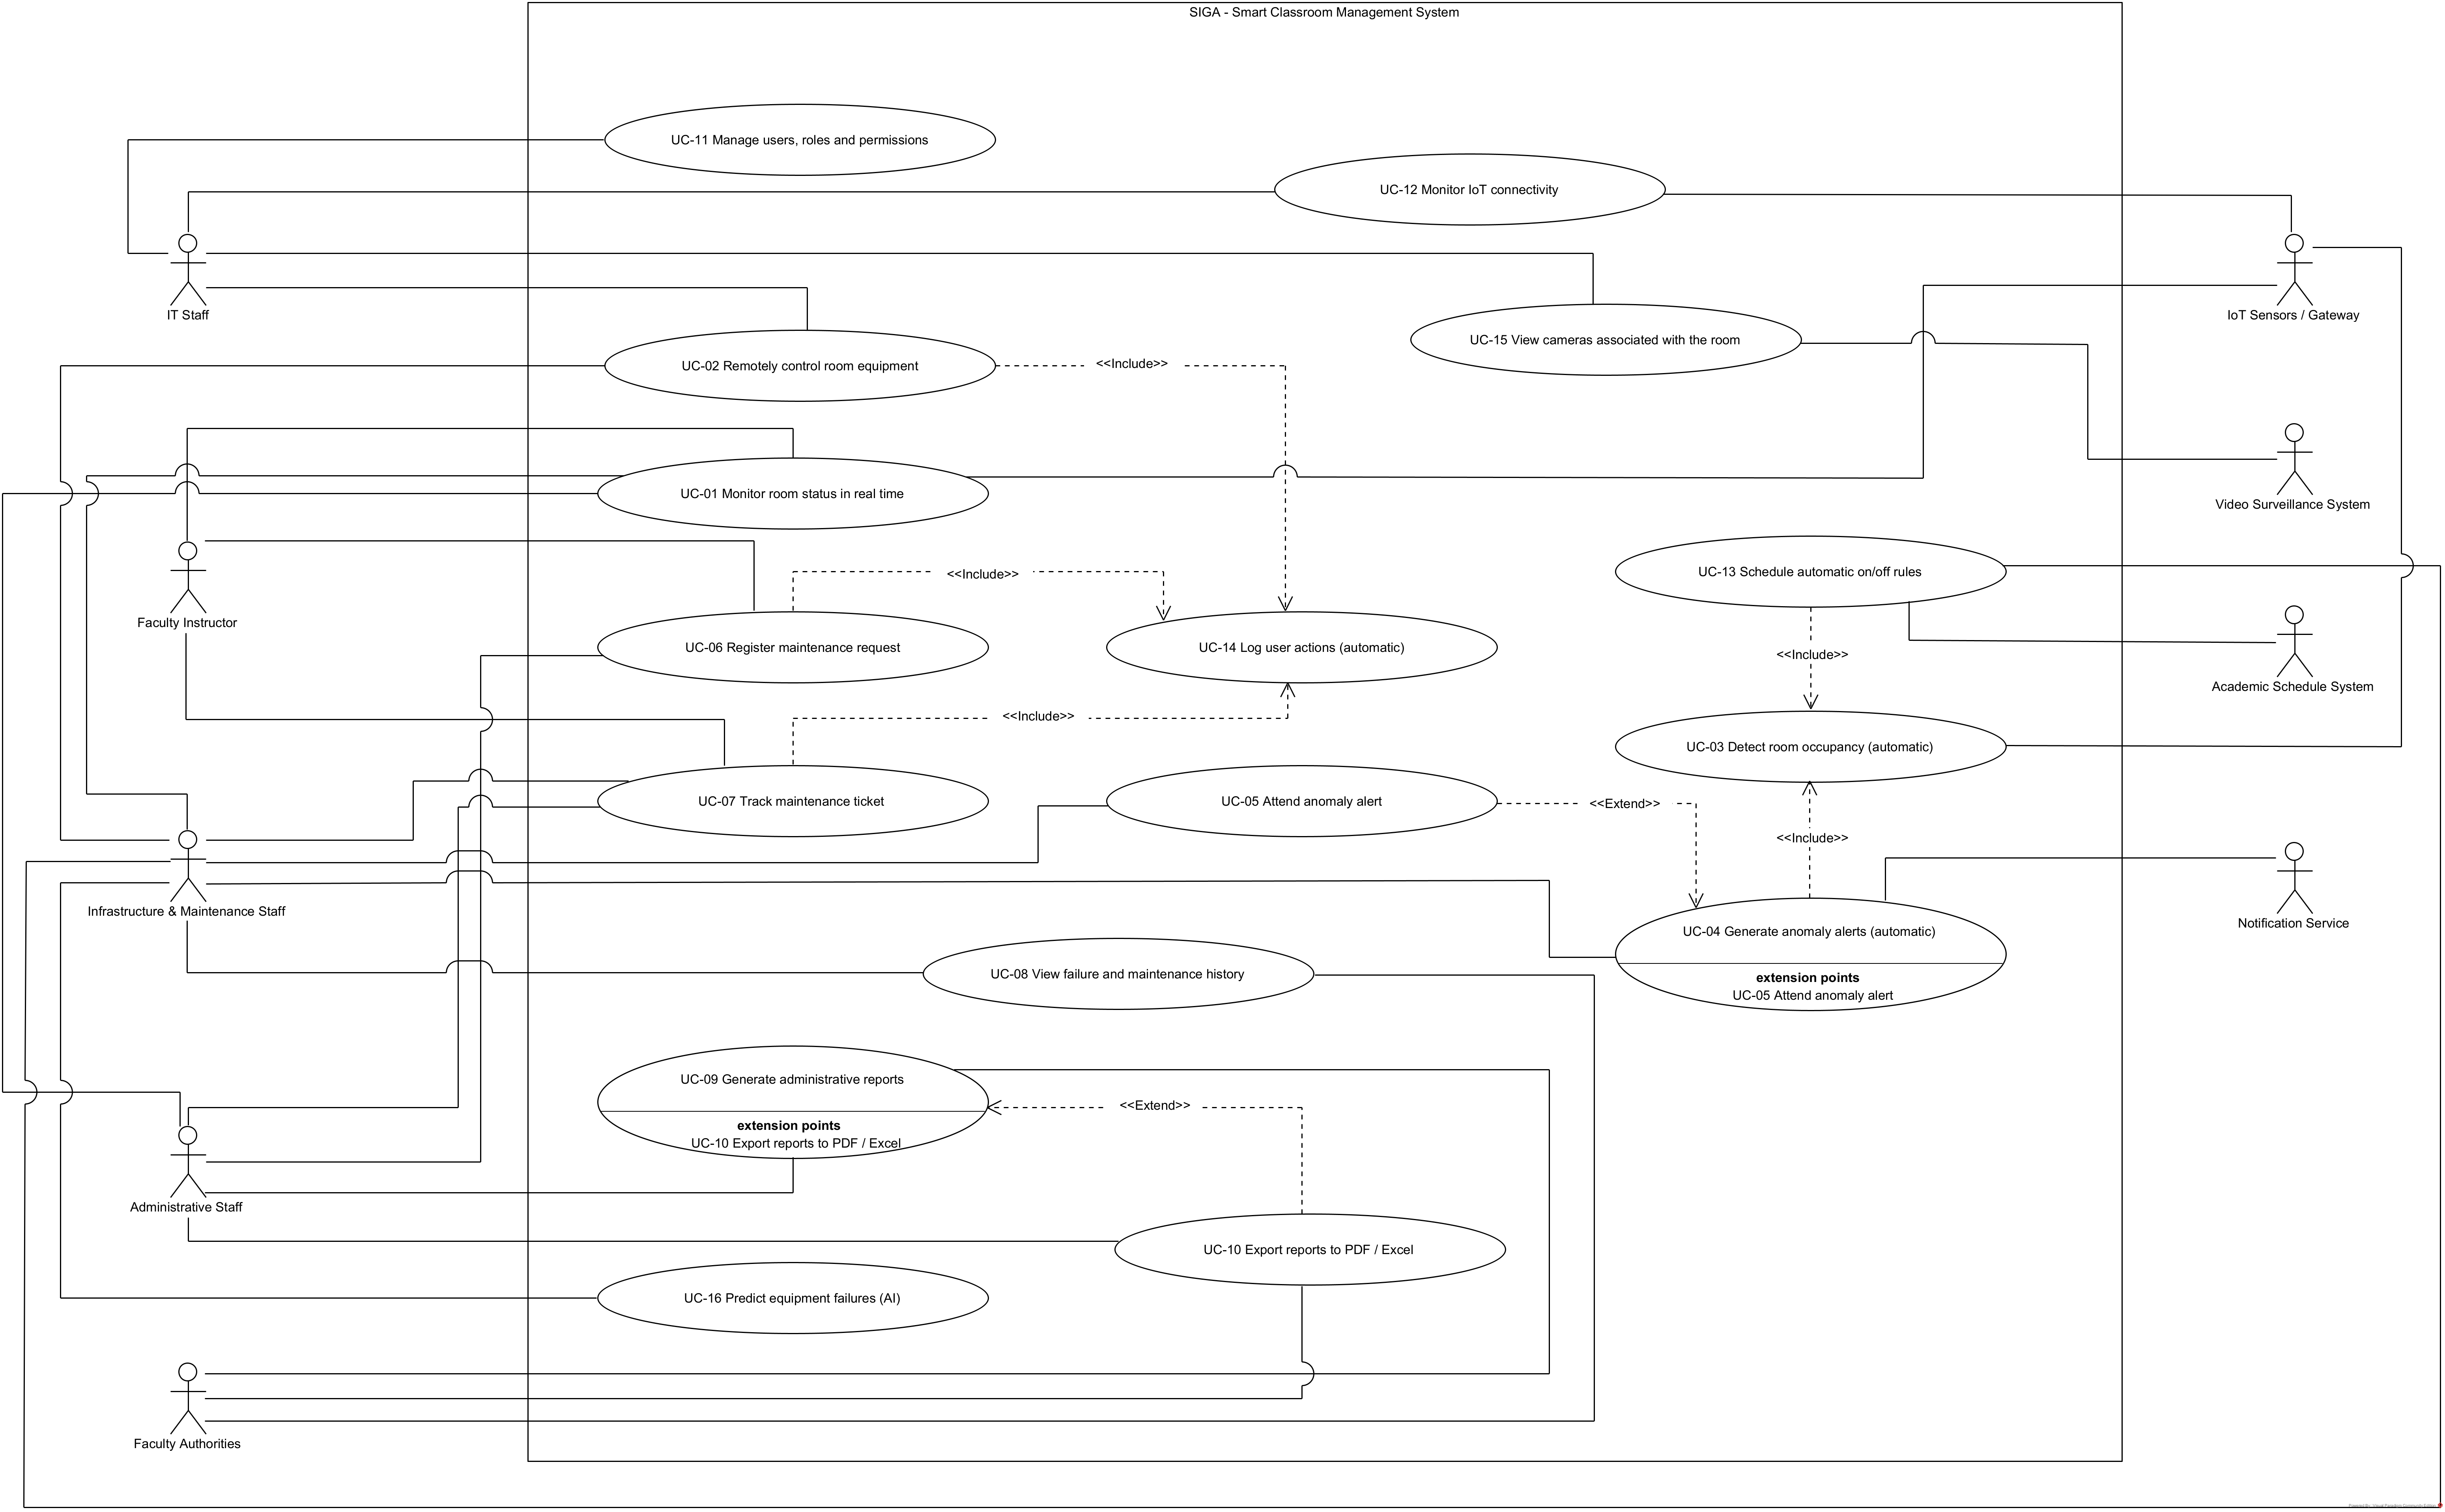
\includegraphics[width=1.25\textwidth]{usecase_general.png}}
\caption{Diagrama general de casos de uso del sistema SIGA}
\label{fig:usecase-general}
\end{figure}

\subsection{Historias de usuario}

Los diecisiete requisitos de prioridad Must tienen historia en formato Connextra con un escenario de aceptaci\'on Gherkin. Las diecisiete se reescribieron por completo en la versi\'on 4.0 (defectos D-10 y D-13). La Tabla~\ref{tab:historias} resume el rol y el beneficio de cada una; el escenario completo est\'a en la \S3.6 del ERS.

\begin{table}[H]
\centering
\small
\begin{tabular}{|l|l|p{2.9cm}|p{6.2cm}|}
\hline
\cellcolor{sigagreen}\textcolor{white}{\textbf{HU}} & \cellcolor{sigagreen}\textcolor{white}{\textbf{RF}} & \cellcolor{sigagreen}\textcolor{white}{\textbf{Rol}} & \cellcolor{sigagreen}\textcolor{white}{\textbf{Beneficio buscado}} \\ \hline
HU-01 & RF-01 & Infraestructura & Conocer el estado de las aulas sin recorrerlas \\ \hline
HU-02 & RF-02 & Infraestructura & No desplazarse hasta el aula para operar equipos \\ \hline
HU-03 & RF-03 & Infraestructura & Activar el ahorro sin revisar c\'amaras manualmente \\ \hline
HU-04 & RF-04 & Infraestructura & Resolver la falla m\'as frecuente sin interrumpir la clase \\ \hline
HU-05 & RF-05 & Infraestructura & Mantener condiciones adecuadas sin desplazarse \\ \hline
HU-06 & RF-07 & Infraestructura & Detectar de un vistazo qu\'e aula necesita atenci\'on \\ \hline
HU-07 & RF-08 & Infraestructura & Enterarse de la anomal\'ia sin vigilar el panel \\ \hline
HU-08 & RF-10 & Infraestructura & Sustentar los informes al decanato con datos \\ \hline
HU-09 & RF-11 & Docente & Que la interrupci\'on se resuelva sin perder la hora \\ \hline
HU-10 & RF-12 & Docente & Saber si el reporte fue recibido y en qu\'e punto est\'a \\ \hline
HU-11 & RF-13 & Infraestructura & No depender de que alguien recorra el edificio \\ \hline
HU-12 & RF-15 & Infraestructura & Que el ahorro no dependa de una acci\'on diaria \\ \hline
HU-13 & RF-16 & Infraestructura & Eliminar el desperdicio energ\'etico nocturno \\ \hline
HU-14 & RF-19 & Personal de TI & Desplegar en producci\'on sin exponer operaciones cr\'iticas \\ \hline
HU-15 & RF-21 & Infraestructura & Corregir el desperdicio que motiv\'o el proyecto \\ \hline
HU-16 & RF-22 & Personal de TI & No decidir con datos desactualizados sin advertirlo \\ \hline
HU-17 & RF-23 & Personal de TI & Auditar qui\'en hizo qu\'e y cu\'ando \\ \hline
\end{tabular}
\caption{Historias de usuario de los requisitos Must}
\label{tab:historias}
\end{table}

Los ocho requisitos de prioridad Should no llevan historia ni criterio BDD, porque la gu\'ia los exige \'unicamente para los Must. Esa ausencia est\'a marcada como tal en la matriz de trazabilidad, con su raz\'on, y no como una cadena rota.

\subsection{Requisitos legales}

El sistema trata datos personales, por lo que el ERS mapea cada obligaci\'on relevante de la Ley Org\'anica de Protecci\'on de Datos Personales del Ecuador \cite{asamblea2021lopdp} al requisito que la operacionaliza: el Art. 13 (derecho de acceso) origina RF-24 y NFR-11; el Art. 14 (rectificaci\'on) origina RF-25; el deber de responsabilidad demostrada de los Art. 10 lit. k y 47 num. 2 se apoya en la bit\'acora de RF-23; y la notificaci\'on de vulneraciones de los Art. 43 y 46 se apoya en NFR-12. La \S3.4 del ERS argumenta adem\'as por qu\'e el procesamiento de imagen para determinar presencia agregada no constituye dato biom\'etrico en los t\'erminos del Art. 4, lo que sustenta la clasificaci\'on del proyecto en Categor\'ia B de riesgo \'etico.

\subsection{Restricciones de dise\~no}

Dieciocho restricciones acotan el espacio de soluci\'on en cinco ejes: tecnol\'ogico (RD-01 a RD-06: protocolos IoT, red institucional, base de datos aprobada, compatibilidad de equipos, l\'imite de la integraci\'on con videovigilancia y ejecuci\'on en navegador), econ\'omico (RD-07 y RD-08: presupuesto de hardware y despliegue por aulas piloto), normativo (RD-09 a RD-11: protecci\'on de datos, acceso por roles y bit\'acora), operativo (RD-12 y RD-13: dependencia del personal de Infraestructura y del horario acad\'emico digital), temporal (RD-14 y RD-15) y de alcance (RD-16 a RD-18, que fijan por escrito lo que el sistema no har\'a).

\subsection{Qu\'e cambi\'o en la versi\'on 4.0}

\begin{table}[H]
\centering
\small
\begin{tabular}{|p{4.3cm}|p{8.4cm}|l|}
\hline
\cellcolor{sigagreen}\textcolor{white}{\textbf{Cambio}} & \cellcolor{sigagreen}\textcolor{white}{\textbf{Motivo}} & \cellcolor{sigagreen}\textcolor{white}{\textbf{Defecto}} \\ \hline
RNF-17, seguridad f\'isica & El modelo de calidad no cubr\'ia \emph{Safety} pese a que el sistema emite comandos de apagado sobre equipos f\'isicos & D-04 \\ \hline
CU-17, derechos sobre datos & RF-24 y RF-25 colgaban de CU-11, cuyo prop\'osito es la gesti\'on de acceso, no el ejercicio de derechos & D-07 \\ \hline
\S4.11, DFD de nivel 1 & Ning\'un modelo describ\'ia el flujo de datos a nivel de proceso, eslab\'on exigido por la cadena de trazabilidad & D-08 \\ \hline
Prioridad de 13 RNF & Solo cuatro RNF ten\'ian prioridad MoSCoW declarada & D-02 \\ \hline
Reescritura de 17 historias & Connextra malformado y cl\'ausula \emph{Cuando} sin evento observable & D-10, D-13 \\ \hline
\S6.1, alcance del MVP & Las secciones 6.1 y 6.4 declaraban conjuntos distintos de RF; solo siete coincid\'ian & D-12 \\ \hline
Reclasificaci\'on de NFR-05 y NFR-15 & Usaban \emph{Portabilidad}, caracter\'istica que ISO/IEC 25010:2023 sustituy\'o por \emph{Flexibilidad} & D-14 \\ \hline
\end{tabular}
\caption{Cambios incorporados en la versi\'on 4.0 del ERS}
\label{tab:cambios-v4}
\end{table}

Los siete cambios provienen de la auditor\'ia de calidad (\S5), no de una revisi\'on editorial: cada uno cierra un defecto registrado con su ubicaci\'on exacta en el documento.

\section{Modelos UML}

El conjunto completo de modelos reside en el ERS (\S\ref{sec:ers-final}) y como archivos individuales en \texttt{03\_Modelado/}, en formato editable y exportado. Esta secci\'on no los reproduce: los lee. La gu\'ia pide para este apartado una \emph{lectura interpretativa}, y eso es lo que sigue: qu\'e decisi\'on de ingenier\'ia sostiene cada modelo, qu\'e revela que los otros no muestran, y d\'onde los modelos se contradicen entre s\'i o con el texto.

\subsection{Qu\'e sostiene cada modelo}

La Tabla~\ref{tab:modelos-decision} resume, para cada modelo, la pregunta que responde y la decisi\'on de ingenier\'ia que sostiene.

\begin{table}[H]
\centering
\small
\begin{tabular}{|p{3.4cm}|p{5.6cm}|p{5.0cm}|}
\hline
\cellcolor{sigagreen}\textcolor{white}{\textbf{Modelo}} & \cellcolor{sigagreen}\textcolor{white}{\textbf{Pregunta que responde}} & \cellcolor{sigagreen}\textcolor{white}{\textbf{Decisi\'on que sostiene}} \\ \hline
Contexto & Qu\'e queda dentro y qu\'e fuera del sistema & Las cuatro exclusiones de RD-16 a RD-18 \\ \hline
Casos de uso (17) & Qu\'e puede hacer cada actor & El reparto de permisos de RF-19 \\ \hline
Clases refinadas (16) & Qu\'e entidades persisten y c\'omo se relacionan & La jerarqu\'ia \texttt{Equipo} y el acoplamiento que mide M5 \\ \hline
Secuencia (16) & En qu\'e orden colaboran los objetos & Los umbrales de latencia de NFR-01 y de los RF de control \\ \hline
Actividad (16) & Qu\'e decisiones y bifurcaciones tiene cada flujo & Los flujos alternativos de cada caso de uso \\ \hline
Estados (2) & Qu\'e ciclo de vida tienen las entidades no triviales & La columna \texttt{Estado} de la matriz de trazabilidad \\ \hline
Componentes & C\'omo se reparte la l\'ogica en m\'odulos & La estructura de m\'odulos del MVP \\ \hline
Despliegue & D\'onde se ejecuta cada parte & Las dependencias DEP-01 a DEP-09 \\ \hline
i* SD y SR & Por qu\'e cada actor quiere lo que quiere & La justificaci\'on de prioridad de los RF n\'ucleo \\ \hline
DFD nivel 1 & Por d\'onde circulan los datos & El eslab\'on \texttt{Proceso} de la cadena de trazabilidad \\ \hline
\end{tabular}
\caption{Modelos del sistema y decisi\'on de ingenier\'ia que cada uno sostiene}
\label{tab:modelos-decision}
\end{table}

\subsection{Lectura del modelo de clases}

El modelo refina diecis\'eis clases: \texttt{Aula}, \texttt{SensorIoT}, \texttt{LecturaSensor}, \texttt{Equipo}, \texttt{Proyector}, \texttt{Climatizador}, \texttt{GatewayIoT}, \texttt{Alerta}, \texttt{SolicitudMantenimiento}, \texttt{Usuario}, \texttt{Rol}, \texttt{HorarioAcademico}, \texttt{ConsumoEnergetico}, \texttt{ReporteAdministrativo}, \texttt{BitacoraAccion} y \texttt{CamaraVigilancia}.

La decisi\'on estructural m\'as relevante es la \textbf{jerarqu\'ia de herencia} \texttt{Equipo} $\rightarrow$ \{\texttt{Proyector}, \texttt{Climatizador}\}. No es cosm\'etica: es lo que permite que RF-02 (control remoto de dispositivos) se especifique una sola vez y que RF-04 y RF-05 sean casos concretos suyos sobre subtipos, en lugar de tres requisitos de control independientes que habr\'ia que mantener en paralelo. La alternativa descartada era modelar proyector y climatizador como clases sin relaci\'on, con un atributo \texttt{tipo} discriminante; se descart\'o porque obligaba a duplicar las operaciones de control y porque romp\'ia la extensibilidad que exige NFR-09 (incorporar un nuevo tipo de dispositivo sin tocar el n\'ucleo).

La segunda lectura relevante es de \textbf{acoplamiento}, y es la que explica la \'unica m\'etrica que no cumple. Dos clases concentran las relaciones: \texttt{Aula}, que participa en pr\'acticamente todo flujo de monitoreo, y \texttt{Equipo}, que participa en todo flujo de control. Por eso, al muestrear la modificabilidad (\S8), RF-01 y RF-07 arrastran seis requisitos cada uno. Ese acoplamiento no es un error de especificaci\'on sino una propiedad del dominio: un aula es, literalmente, el agregado que contiene todo lo dem\'as, pero tiene una consecuencia pr\'actica que conviene declarar: cualquier cambio en la definici\'on de \texttt{Aula} o en la de \texttt{LecturaSensor} obliga a revisar la mitad del cat\'alogo funcional.

\subsection{Lectura de los diagramas de estados}

Solo dos entidades tienen ciclo de vida modelado: \texttt{Alerta} (Generada $\rightarrow$ Notificada $\rightarrow$ \{Atendida $\mid$ Escalada\}) y \texttt{SolicitudMantenimiento} (Registrada $\rightarrow$ En atenci\'on $\rightarrow$ Cerrada). La pregunta pertinente no es por qu\'e hay dos, sino por qu\'e no hay m\'as, y la respuesta es un criterio expl\'icito: se modela el estado de una entidad cuando su comportamiento depende de su historia, no de su valor actual. Un \texttt{Aula} est\'a ocupada o vac\'ia seg\'un su \'ultima lectura, sin memoria; una \texttt{Alerta}, en cambio, no puede escalarse si no fue notificada antes. Aplicar el criterio al rev\'es (modelar un estado por cada clase) habr\'ia producido nueve diagramas triviales sin valor de verificaci\'on.

Esa decisi\'on tiene una consecuencia directa sobre la trazabilidad: la columna \texttt{Estado} de la matriz aparece como \emph{no aplica} en la mayor\'ia de las filas, y eso se declara con su raz\'on en cada una. La plantilla de la gu\'ia lo prev\'e expresamente al definir esa columna como aplicable ``si aplica''.

La transici\'on \texttt{Notificada} $\rightarrow$ \texttt{Escalada} merece atenci\'on aparte porque es la \'unica que se dispara por tiempo y no por acci\'on de un actor: ocurre cuando transcurre el umbral sin atenci\'on. Es, por tanto, el punto donde el modelo de estados y NFR-01 se tocan, y donde un cambio en el umbral de la alerta obliga a revisar ambos artefactos.

\subsection{Lectura del modelado organizacional i*}

Los diagramas i* responden una pregunta que ni los casos de uso ni las clases responden: \emph{por qu\'e} cada actor quiere lo que pide. El diagrama de Dependencia Estrat\'egica muestra que el Docente no depende del sistema, sino del Personal de Infraestructura, y que es este \'ultimo quien depende de SIGA para obtener datos de sensor en tiempo real. Esa cadena (Docente $\rightarrow$ Infraestructura $\rightarrow$ SIGA) explica un hecho que de otro modo parecer\'ia un descuido de elicitaci\'on: el Docente figura como origen de nueve requisitos pero casi nunca como usuario operativo del sistema. No es que se le haya ignorado; es que su dependencia est\'a mediada.

El diagrama de Raz\'on Estrat\'egica descompone el \emph{softgoal} ``reducir el tiempo de respuesta a fallas'' del Personal de Infraestructura en tres tareas que se corresponden con RF-07, RF-08 y RF-12. Esa descomposici\'on es la justificaci\'on documentada de por qu\'e esos tres requisitos son Must: no lo son por criterio del equipo, sino porque son las tres tareas en que se descompone el objetivo del actor con mayor poder e inter\'es del mapa de \emph{stakeholders}.

\subsection{CU-17: Ejercer derechos sobre datos personales (nuevo)}

RF-24 (exportaci\'on de datos personales) y RF-25 (rectificaci\'on) exist\'ian desde la Entrega 3, derivados del an\'alisis de los Art. 13 y 14 de la LOPDP, pero no ten\'ian caso de uso propio: colgaban impl\'icitamente de CU-11, cuyo prop\'osito es la gesti\'on de acceso por roles. Son cosas distintas: CU-11 responde a ``qui\'en puede entrar y a qu\'e'', mientras que el ejercicio de derechos responde a ``qu\'e puede exigir el titular sobre sus propios datos'', con actores, plazos legales y evidencia diferentes. Mientras esa confusi\'on persisti\'o, ambos requisitos figuraban como hu\'erfanos de caso de uso en el diagn\'ostico de trazabilidad.

CU-17 lo corrige: actor principal Docente, actores secundarios Personal Administrativo y de TI, con un curso normal que cubre las dos v\'ias (acceso y rectificaci\'on), el plazo de $\leq$15 d\'ias h\'abiles de NFR-11 y el registro en bit\'acora que permite demostrar cumplimiento ante la Autoridad de Protecci\'on de Datos. Su flujo alternativo A3 es deliberadamente conservador: cuando el plazo est\'a por vencer, el sistema alerta al responsable pero \textbf{no} resuelve la solicitud por su cuenta, porque una respuesta autom\'atica a un derecho del titular no ser\'ia defendible ante la autoridad.

\subsection{Diagrama de Flujo de Datos: Nivel 1 (nuevo)}

El ERS de la Entrega 3 modelaba estructura y comportamiento, pero ning\'un modelo describ\'ia el flujo de datos a nivel de proceso. Ese vac\'io no era cosm\'etico: el proceso DFD es un eslab\'on de la cadena de trazabilidad que la gu\'ia exige, y sin \'el ninguna cadena adelante pod\'ia cerrarse, que es la causa de que M4\_ade midiera 0\,\% en la primera auditor\'ia (\S8).

Los ocho procesos (Tabla~\ref{tab:dfd-procesos}) se derivaron agrupando los RF que comparten el mismo flujo de entrada y salida, verificado contra la matriz de trazabilidad; no provienen de una plantilla gen\'erica.

\begin{table}[H]
\centering
\small
\begin{tabular}{|l|p{5.5cm}|p{5.2cm}|}
\hline
\cellcolor{sigagreen}\textcolor{white}{\textbf{Proceso}} & \cellcolor{sigagreen}\textcolor{white}{\textbf{Nombre}} & \cellcolor{sigagreen}\textcolor{white}{\textbf{RF que agrupa}} \\ \hline
P-1 & Captura de datos ambientales y ocupaci\'on & RF-01, RF-03, RF-20, RF-22 \\ \hline
P-2 & Control remoto de equipos & RF-02, RF-04, RF-05 \\ \hline
P-3 & Generaci\'on y gesti\'on de alertas & RF-08, RF-11, RF-21 \\ \hline
P-4 & Automatizaci\'on energ\'etica & RF-13, RF-15, RF-16 \\ \hline
P-5 & Gesti\'on de mantenimiento & RF-10, RF-12 \\ \hline
P-6 & Reportes administrativos & RF-14, RF-17, RF-18 \\ \hline
P-7 & Gesti\'on de acceso y auditor\'ia & RF-19, RF-23 \\ \hline
P-8 & Gesti\'on de derechos sobre datos personales & RF-24, RF-25 \\ \hline
\end{tabular}
\caption{Procesos del DFD de nivel 1}
\label{tab:dfd-procesos}
\end{table}

El diagrama hace visibles dos cosas que ning\'un modelo anterior mostraba. La primera es que el almac\'en de bit\'acora (D4) recibe escrituras de \textbf{seis de los ocho procesos}. Es coherente con RF-23 y con el deber de responsabilidad demostrada de la LOPDP, pero convierte a ese almac\'en en un punto \'unico de fallo para la auditabilidad de todo el sistema: si la escritura en bit\'acora falla silenciosamente, el sistema sigue operando con normalidad y la p\'erdida solo se descubre cuando alguien pide la evidencia. Ning\'un requisito actual cubre ese escenario, y se deja anotado como candidato para la siguiente iteraci\'on.

La segunda es que P-8 no exist\'ia como proceso en ninguna vista previa, lo que confirma desde un \'angulo independiente el mismo problema que motiv\'o CU-17: el ejercicio de derechos del titular estaba disuelto dentro de la gesti\'on de acceso.

\subsection{Coherencia entre modelos}

Un conjunto de modelos puede ser individualmente correcto y colectivamente incoherente, de modo que se verificaron tres correspondencias que deb\'ian cumplirse por construcci\'on:

\begin{itemize}
\item \textbf{Casos de uso frente a clases.} Toda clase del modelo de dominio participa en al menos un caso de uso, y todo caso de uso referencia al menos una clase. Se comprob\'o sobre la matriz de trazabilidad, columna \texttt{Clase\_UML}.
\item \textbf{Casos de uso frente a actores.} Los nueve actores del diagrama general participan en al menos un caso de uso, desde Personal de Infraestructura, presente en diez, hasta el Sistema de Videovigilancia, presente solo en CU-15. Ese conteo es el que sustenta la m\'etrica M1c (\S8).
\item \textbf{Procesos DFD frente a requisitos.} Los 25 RF est\'an cubiertos por exactamente uno de los ocho procesos, sin solapamiento ni hueco. Los RF de IA se adscriben al proceso del RF que refinan.
\end{itemize}

La \'unica incoherencia detectada entre modelos y texto durante esta verificaci\'on fue la ausencia f\'isica de una figura de diagrama de estados que el ERS referenciaba (defecto D-11): el archivo exist\'ia en la carpeta de modelado pero no en la de figuras del documento, de modo que el modelo estaba, y lo que faltaba era su v\'inculo.

\section{Validaci\'on}

\subsection{Naturaleza de esta inspecci\'on}

No exist\'ia en el repositorio ning\'un registro de defectos ni de inspecci\'on de ninguna entrega anterior. Esta secci\'on documenta la \textbf{primera} inspecci\'on formal realizada sobre el ERS, ejecutada entre el 20 y el 22 de agosto de 2026 sobre la versi\'on 3.0 (commit \texttt{9f7c54c}), y la re-inspecci\'on posterior a las correcciones sobre la versi\'on 4.0. El registro completo, con ubicaci\'on de cada hallazgo y la acci\'on tomada, est\'a en \texttt{09\_Metricas/registro\_defectos.csv}; la aritm\'etica de las m\'etricas derivadas, en \texttt{09\_Metricas/Anexo\_A\_Auditoria\_Calidad\_ERS\_SIGA.md} y en \S8.

\subsection{M\'etodo de inspecci\'on}

La inspecci\'on no fue una lectura general en busca de errores, sino un recorrido con criterios fijados de antemano. Se aplicaron cuatro pasadas sobre el documento:

\begin{enumerate}
\item \textbf{Completitud de atributos.} Para cada uno de los 42 requisitos se comprob\'o la presencia de los cuatro atributos obligatorios: identificador, prioridad, fuente y criterio de aceptaci\'on, contando campos no vac\'ios. Esta pasada produjo D-02.
\item \textbf{Verificabilidad.} A cada criterio de aceptaci\'on se le aplicaron las cuatro preguntas de la gu\'ia: si existe umbral num\'erico o resultado observable, si est\'a definida la unidad, si se indica el m\'etodo de comprobaci\'on, y si dos evaluadores independientes llegar\'ian al mismo veredicto. Complementariamente se busc\'o de forma autom\'atica el vocabulario no medible habitual.
\item \textbf{Coherencia entre declaraciones duplicadas.} Cada dato que aparece m\'as de una vez en el proyecto (la prioridad de un requisito, el n\'umero de requisitos de cada tipo, el alcance del MVP, la caracter\'istica de calidad de cada RNF) se contrast\'o entre todas sus apariciones. Esta pasada produjo los tres defectos de contradicci\'on: D-01, D-12 y D-14.
\item \textbf{Integridad de la cadena de trazabilidad.} Se recorri\'o cada requisito de la fuente al caso de prueba, marcando el eslab\'on donde la cadena se interrumpe. Esta pasada produjo D-05, D-07, D-08 y D-09.
\end{enumerate}

Un defecto se registr\'o solo cuando pod\'ia se\~nalarse su ubicaci\'on exacta en el documento. Las impresiones sin ubicaci\'on verificable no entraron al registro, porque un defecto que no se puede mostrar tampoco se puede corregir ni contar.

\subsection{Clasificaci\'on adoptada y su efecto en la medici\'on}

Los defectos se clasificaron en cuatro tipos (Tabla~\ref{tab:tipos-defecto}), y esa clasificaci\'on determina cu\'ales entran en la m\'etrica de correcci\'on:

\begin{table}[H]
\centering
\small
\begin{tabular}{|l|p{7.6cm}|c|}
\hline
\cellcolor{sigagreen}\textcolor{white}{\textbf{Tipo}} & \cellcolor{sigagreen}\textcolor{white}{\textbf{Criterio}} & \cellcolor{sigagreen}\textcolor{white}{\textbf{Cuenta para M6}} \\ \hline
Contradicci\'on & El documento afirma dos cosas incompatibles sobre el mismo elemento & S\'i \\ \hline
Atributo faltante & Un requisito existente carece de un atributo obligatorio & S\'i \\ \hline
Ambig\"uedad & Un enunciado existente admite m\'as de una lectura o no es comprobable & S\'i \\ \hline
Artefacto faltante & Un producto de trabajo que la Unidad V manda construir no exist\'ia a\'un & No \\ \hline
\end{tabular}
\caption{Tipos de defecto y su inclusi\'on en la m\'etrica de correcci\'on}
\label{tab:tipos-defecto}
\end{table}

La distinci\'on de la \'ultima fila es la m\'as importante y conviene justificarla, porque infla o desinfla la m\'etrica seg\'un c\'omo se decida. La m\'etrica de correcci\'on mide \emph{defectos residuales que sobreviven a la inspecci\'on} sobre el documento ya corregido. Un DFD que no exist\'ia no es un defecto del ERS de la Entrega 3: es un entregable que la Unidad V pide construir en su Paso 2. Contarlo como defecto habr\'ia elevado artificialmente el valor ``antes'' y hecho parecer m\'as espectacular la mejora. Contarlo aparte, como se hace aqu\'i, deja la m\'etrica midiendo lo que dice medir.

\subsection{Defectos hallados y estado al cierre}

\begin{table}[H]
\centering
\small
\begin{tabular}{|l|l|l|p{5.6cm}|c|c|l|}
\hline
\textbf{ID} & \textbf{Tipo} & \textbf{Sever.} & \textbf{Descripci\'on} & \textbf{Inst.} & \textbf{M6} & \textbf{Estado} \\ \hline
D-01 & Contradicci\'on & Cr\'itica & Prioridad MoSCoW de RF-20/24/25 distinta entre el documento y el CSV de priorizaci\'on & 3 & S\'i & Resuelto \\ \hline
D-02 & Atributo falt. & Alta & Doce RNF sin prioridad MoSCoW declarada en ning\'un lugar & 12 & S\'i & Resuelto \\ \hline
D-03 & Limitaci\'on & Media & Solo 2 de 9 actores figuran como fuente de alg\'un RF & 7 & No & Declarado \\ \hline
D-04 & Vac\'io normativo & Alta & Ninguna caracter\'istica Safety pese al apagado autom\'atico f\'isico & 1 & No & Resuelto \\ \hline
D-05 & Artefacto falt. & Cr\'itica & Cero casos de prueba conceptual & 25 & No & Resuelto \\ \hline
D-06 & Artefacto falt. & Media & RF Must sin historia de usuario ni Gherkin & 3 & S\'i & Resuelto \\ \hline
D-07 & Artefacto falt. & Media & Sin CU dedicado a los derechos LOPDP & 1 & No & Resuelto \\ \hline
D-08 & Artefacto falt. & Cr\'itica & Sin Diagrama de Flujo de Datos & 1 & No & Resuelto \\ \hline
D-09 & Artefacto falt. & Alta & Los RNF ausentes de la matriz de trazabilidad & 16 & S\'i & Resuelto \\ \hline
D-10 & Ambig\"uedad & Media & Cl\'ausula Gherkin ``Cuando'' sin evento observable & 17 & S\'i & Resuelto \\ \hline
D-11 & Artefacto falt. & Alta & Imagen de diagrama de estados referenciada e inexistente & 1 & No & Resuelto \\ \hline
D-12 & Contradicci\'on & Alta & \S6.1 y \S6.4 con conjuntos distintos de RF para el MVP & 1 & S\'i & Resuelto \\ \hline
D-13 & Ambig\"uedad & Media & Connextra malformado en las 17 historias de usuario & 17 & S\'i & Resuelto \\ \hline
D-14 & Contradicci\'on & Media & Dos RNF clasificados bajo \emph{Portabilidad}, caracter\'istica que ISO/IEC 25010:2023 sustituy\'o por \emph{Flexibilidad} & 2 & S\'i & Resuelto \\ \hline
D-15 & Contradicci\'on & Alta & Diagrama de estados de \texttt{Alerta} con un ciclo distinto del especificado en la \S4.6 del ERS, sin estado \texttt{Escalada} & 1 & S\'i & Resuelto \\ \hline
\end{tabular}
\caption{Registro de defectos de la inspecci\'on PE5 y su estado al cierre}
\label{tab:defectos}
\end{table}

\subsection{Correcciones aplicadas}

\begin{itemize}
\item \textbf{D-01.} Resuelto a favor del documento: RF-20, RF-24 y RF-25 quedan Should, versi\'on coherente con cuatro secciones del ERS, con el \texttt{CHANGELOG} y con el README del MVP. La priorizaci\'on se consolid\'o en un \'unico archivo (17 Must, 8 Should) y se elimin\'o el duplicado que manten\'ia viva la contradicci\'on dentro del repositorio.
\item \textbf{D-02.} Se declar\'o la prioridad de los 13 RNF pendientes en la Tabla 42, cada una con justificaci\'on escrita.
\item \textbf{D-04.} RNF-17 (seguridad f\'isica) redactado y fusionado en la Tabla 39. Se numera 17 y no 16 para no colisionar con el NFR-16 preexistente, que trata la disponibilidad en modo degradado y tiene evidencia de campo propia (EV-15).
\item \textbf{D-05.} Cuarenta y dos casos de prueba conceptuales, cada uno derivado del criterio de verificaci\'on real de su requisito.
\item \textbf{D-06.} Disuelto al cerrar D-01: los tres RF son Should y la gu\'ia exige historia y criterio BDD solo para los Must. Verificado por script que los 17 Must tienen historia.
\item \textbf{D-07 y D-08.} CU-17 fusionado en la \S4.2 del ERS y DFD de nivel 1 como \S4.11.
\item \textbf{D-09.} Matriz PE5 de 48 filas, con los 17 RNF y los 6 RF de IA.
\item \textbf{D-10 y D-13.} Las 17 historias reescritas por completo: cl\'ausula Connextra con rol, funcionalidad y beneficio diferenciados, y escenario Gherkin cuyo ``Cuando'' nombra el evento concreto que lo dispara.
\item \textbf{D-11.} Figura restituida desde \texttt{03\_Modelado/}.
\item \textbf{D-12.} La \S6.1 se reescribi\'o declarando el alcance planificado, la desviaci\'on y su causa: cinco RF pospuestos por depender de hardware no disponible y cuatro sustituidos por otros demostrables con el simulador. Se fija la cifra de \S6.4 (11/17, 64,7\,\%) como cobertura real verificada contra c\'odigo.
\end{itemize}

\subsection{Lo que no se corrigi\'o y por qu\'e}

\textbf{D-03} se reclasific\'o de defecto a \textbf{limitaci\'on declarada}. Bajo la definici\'on de cobertura adoptada para M1c (\S8), los nueve actores participan en al menos un caso de uso, de modo que no hay un vac\'io de completitud en el documento. Lo que s\'i persiste, y se declara, es una \textbf{concentraci\'on real de las fuentes de elicitaci\'on}: siete de los nueve actores nunca fueron entrevistados como origen de un requisito, lo que afecta la validez externa del ERS y solo se resuelve con m\'as trabajo de campo, no con edici\'on documental.

Tambi\'en queda pendiente la \textbf{re-inspecci\'on independiente} de la versi\'on 4.0. La verificaci\'on posterior a las correcciones fue automatizada y cubri\'o lo comprobable por script; una re-lectura sem\'antica por una persona distinta de quien aplic\'o las correcciones es lo que respaldar\'ia definitivamente el M6 igual a cero que se reporta en \S8.

\subsection{Resultado de la re-inspecci\'on}

Tras aplicar las correcciones se ejecut\'o una re-inspecci\'on sobre la versi\'on 4.0. La parte automatizable se verific\'o por \emph{script} para que el resultado no dependa del criterio de quien mira; la Tabla~\ref{tab:reinspeccion} recoge qu\'e se comprob\'o y qu\'e devolvi\'o cada comprobaci\'on.

\begin{table}[H]
\centering
\small
\begin{tabular}{|p{6.9cm}|p{3.1cm}|p{3.4cm}|}
\hline
\cellcolor{sigagreen}\textcolor{white}{\textbf{Comprobaci\'on}} & \cellcolor{sigagreen}\textcolor{white}{\textbf{Esperado}} & \cellcolor{sigagreen}\textcolor{white}{\textbf{Obtenido}} \\ \hline
Identificadores RF definidos frente a citados & 25 y sin hu\'erfanos & 25, sin hu\'erfanos \\ \hline
Identificadores RNF definidos & 17 & 17 \\ \hline
Casos de uso con especificaci\'on textual & 17 & 17 \\ \hline
Historias de usuario para los RF Must & 17 de 17 & 17 de 17 \\ \hline
Prioridad MoSCoW: Tabla 42 frente al CSV & Coincidencia en los 42 & Coincidencia en los 42 \\ \hline
Conteos narrativos frente a identificadores reales & Coincidencia & Coincidencia \\ \hline
Casos de prueba citados en la matriz y definidos & Correspondencia en ambos sentidos & Correspondencia total \\ \hline
Filas de la matriz con cadena completa & 48 de 48 & 48 de 48 \\ \hline
Entradas bibliogr\'aficas citadas en el cuerpo & 36 de 36 & 36 de 36 \\ \hline
Entornos de tabla abiertos y cerrados & Balance exacto & Balance exacto \\ \hline
Figuras referenciadas y presentes en disco & Todas & Todas \\ \hline
\end{tabular}
\caption{Comprobaciones automatizadas de la re-inspecci\'on sobre la versi\'on 4.0}
\label{tab:reinspeccion}
\end{table}

Ninguna de estas comprobaciones sustituye a la lectura sem\'antica: verifican que el documento sea internamente coherente, no que lo que afirma sea correcto. Un requisito puede estar bien identificado, bien trazado y bien contado, y aun as\'i describir mal lo que el usuario necesita. Esa es exactamente la distancia que la m\'etrica de correcci\'on no alcanza a medir y que la re-inspecci\'on pendiente deber\'ia cubrir.

\subsection{Una comprobaci\'on emp\'irica de por qu\'e esa re-inspecci\'on hace falta}

La necesidad de esa segunda lectura no es una precauci\'on ret\'orica: se comprob\'o en este mismo trabajo. Los defectos D-13 y D-14 \textbf{no aparecieron en la primera pasada}. D-13 (el Connextra malformado en las diecisiete historias) se detect\'o al reescribir los escenarios Gherkin por D-10, es decir, al mirar el mismo texto con otro prop\'osito. D-14 (dos RNF clasificados bajo una caracter\'istica de calidad que la edici\'on 2023 de la norma ya no contempla) se detect\'o al generar la tabla resumen de \S3, o sea al obligarse a tabular un dato que hasta entonces se hab\'ia le\'ido en prosa.

D-15 confirm\'o el patr\'on por tercera vez, y de la forma m\'as clara. Apareci\'o al final del trabajo, al insertar las figuras en este informe: mientras el diagrama de estados de \texttt{Alerta} solo se citaba en prosa, la contradicci\'on entre el ciclo dibujado y el ciclo especificado era invisible; bast\'o ponerlo en la p\'agina, al lado de su propia descripci\'on, para que saltara. Es un defecto que hab\'ia sobrevivido a dos entregas y a la inspecci\'on formal completa de esta unidad.

El patr\'on es consistente y vale como lecci\'on transferible: en los tres casos el defecto emergi\'o cuando el documento se manipul\'o con una finalidad distinta de la de buscar defectos. Una inspecci\'on que se agota en una \'unica lectura dirigida encuentra lo que su lista de verificaci\'on anticipa, y poco m\'as. Por eso la cifra de correcci\'on que se reporta en \S8 se acompa\~na de su advertencia en lugar de presentarse como un resultado cerrado.

\section{Gesti\'on y trazabilidad}

\subsection{L\'inea base y control de cambios}

La l\'inea base del ERS al iniciar esta unidad es el commit \texttt{9f7c54c} (02/08/2026), \'ultimo cambio real sobre \texttt{01\_ERS/secciones\_generadas.tex}. El trabajo de la Unidad V se versiona en un repositorio propio, \repourl. Las incidencias abiertas est\'an en el registro de defectos (\S5, Tabla~\ref{tab:defectos}); no existi\'o un \emph{Change Control Board} formal documentado en las entregas anteriores, lo que se declara como vac\'io de proceso en vez de fabricar un historial de decisiones que no ocurri\'o.

\subsection{Matriz de trazabilidad final}

La matriz heredada (\texttt{04\_Trazabilidad/matriz\_trazabilidad.csv}, 44 filas) trazaba los 25 RF y 6 restricciones, pero \textbf{ning\'un} RNF (defecto D-09) y no ten\'ia columnas de proceso, estado ni caso de prueba. La matriz PE5 (\texttt{04\_Trazabilidad/matriz\_trazabilidad\_PE5.csv}, \textbf{48 filas}) completa la cadena de la plantilla 7.2 de la gu\'ia con las columnas de la Tabla~\ref{tab:columnas-matriz}:

\begin{table}[H]
\centering
\small
\begin{tabular}{|l|p{9.5cm}|}
\hline
\textbf{Columna} & \textbf{Contenido} \\ \hline
\texttt{ID\_Requisito} & Identificador \'unico (RF, RF-IA o RNF) \\ \hline
\texttt{Fuente} & Evidencia de campo (EV-xx), norma o an\'alisis de origen \\ \hline
\texttt{ID\_CU} & Casos de uso que lo realizan \\ \hline
\texttt{Clase\_UML} & Clases del modelo de dominio implicadas \\ \hline
\texttt{Proceso\_DFD} & Proceso P-1 a P-8 del DFD nivel 1 \\ \hline
\texttt{Estado} & Estado o transici\'on del diagrama de estados, si aplica \\ \hline
\texttt{Criterio\_BDD} & Criterio de aceptaci\'on Dado--Cuando--Entonces \\ \hline
\texttt{ID\_CP} & Caso de prueba conceptual \\ \hline
\texttt{Historia} & Historia del \emph{backlog} \\ \hline
\texttt{Estado\_de\_la\_traza} & Completa o rota, con la acci\'on tomada \\ \hline
\end{tabular}
\caption{Estructura de la matriz de trazabilidad final}
\label{tab:columnas-matriz}
\end{table}

Contenido: los 25 RF, los 6 nuevos RF de IA, los 16 RNF existentes y el nuevo RNF-17.

\begin{table}[H]
\centering
\small
\begin{tabular}{|l|c|c|c|}
\hline
\textbf{Tipo de requisito} & \textbf{Filas} & \textbf{Cadena completa} & \textbf{\%} \\ \hline
RF (RF-01 a RF-25) & 25 & 25 & 100\,\% \\ \hline
RF de IA (RF-IA-01 a RF-IA-06) & 6 & 6 & 100\,\% \\ \hline
RNF (NFR-01 a NFR-16 y RNF-17) & 17 & 17 & 100\,\% \\ \hline
\textbf{Total} & \textbf{48} & \textbf{48} & \textbf{100\,\%} \\ \hline
\end{tabular}
\caption{Diagn\'ostico de cobertura de la matriz PE5}
\label{tab:diagnostico-cobertura}
\end{table}

Las 48 filas cierran cadena completa (Tabla~\ref{tab:diagnostico-cobertura}). En la primera medici\'on eran 35 de 48: las 13 restantes eran RNF, y en doce de los trece casos la causa era la misma, la prioridad MoSCoW no declarada (D-02). Al cerrar ese defecto y redactar los diez casos de prueba de RNF que faltaban, la matriz queda sin filas rotas.

Conviene precisar qu\'e significa aqu\'i ``completa'', porque no todas las columnas aplican a todos los requisitos. Un RNF transversal como NFR-02 (disponibilidad mensual) no se realiza en ning\'un caso de uso ni clase de dominio, y as\'i se declara en su fila: su cadena se cierra por fuente, proceso y caso de prueba, no por caso de uso. Del mismo modo, los RF de prioridad Should no llevan historia ni criterio BDD, porque la gu\'ia los exige solo para los Must. Esas ausencias est\'an marcadas como ``N/A'' con su raz\'on, no como enlaces vac\'ios.

\subsection{Casos de prueba conceptuales}

El ERS no conten\'ia ninguno. Se redactaron \textbf{42}, recogidos en el archivo \texttt{casos\_prueba\_\allowbreak conceptuales.csv} de la carpeta \texttt{04\_Trazabilidad/}, con el formato precondici\'on / acci\'on / resultado esperado y una columna de origen que cita, para cada uno, el criterio de verificaci\'on del ERS del que se deriva. Cubren los 25 RF, los 6 RF de IA y los 17 RNF (diez de ellos con caso propio; los otros siete se verifican junto con el RF con el que comparten umbral). Ejemplo (CP-13, derivado de RF-13): dado un horario cargado y una regla de apagado activa, al simular un aula desocupada fuera de horario, el apagado autom\'atico debe activarse en $\leq$2 minutos y el evento quedar registrado para auditor\'ia.

\subsection{Hu\'erfanos y cadenas rotas}

El cat\'alogo completo est\'a en \texttt{04\_Trazabilidad/huerfanos\_y\_cadenas\_rotas.csv}: 31 entradas, cada una con causa y acci\'on tomada, y ninguna en estado ambiguo. Trece se cerraron como \emph{enlazado} en esta unidad: entre ellas RF-24 y RF-25, que eran hu\'erfanos de caso de uso (colgaban impl\'icitamente de CU-11, que es gesti\'on de acceso y no derechos ARCO) y ahora se realizan en CU-17 y en el proceso P-8 del DFD. El resto queda como \emph{justificado} con su pendiente declarado.

\subsection{Sincronizaci\'on con el \emph{product backlog}}

El equipo no declar\'o formalmente una herramienta de tablero en ninguna entrega anterior verificable en el repositorio, y no se enlaza aqu\'i un tablero inexistente. Lo que s\'i puede verificarse y cuantificarse es la sincronizaci\'on entre el cat\'alogo de requisitos y el conjunto de historias, que es la propiedad que la sincronizaci\'on con el \emph{backlog} persigue: que cada requisito priorizado tenga historia y que cada historia apunte a un requisito existente.

\begin{table}[H]
\centering
\small
\begin{tabular}{|p{7.4cm}|c|c|}
\hline
\cellcolor{sigagreen}\textcolor{white}{\textbf{Comprobaci\'on de sincronizaci\'on}} & \cellcolor{sigagreen}\textcolor{white}{\textbf{Resultado}} & \cellcolor{sigagreen}\textcolor{white}{\textbf{\%}} \\ \hline
RF de prioridad Must con historia asociada & 17 de 17 & 100\,\% \\ \hline
Historias que apuntan a un RF existente & 17 de 17 & 100\,\% \\ \hline
Historias hu\'erfanas, sin RF de origen & 0 & 0\,\% \\ \hline
RF de prioridad Should sin historia & 8 de 8 & no exigido \\ \hline
Requisitos con caso de prueba asociado & 48 de 48 & 100\,\% \\ \hline
\end{tabular}
\caption{Sincronizaci\'on cuantificada entre el cat\'alogo de requisitos y el conjunto de historias}
\label{tab:sincronizacion}
\end{table}

La cuarta fila de la Tabla~\ref{tab:sincronizacion} no es un incumplimiento: la gu\'ia exige historia y criterio BDD solo para los requisitos Must, y los ocho Should quedan deliberadamente sin ella, marcados como tales en la matriz. Lo que falta, y se declara, es el soporte en una herramienta de gesti\'on: la correspondencia est\'a verificada sobre los artefactos del repositorio, no sobre un tablero con estados y responsables. Montarlo queda como acci\'on pendiente.

\subsection{An\'alisis de impacto}

La utilidad pr\'actica de una matriz de trazabilidad no es documental sino predictiva: sirve para responder, antes de aceptar un cambio, qu\'e habr\'ia que revisar si ese cambio se aprueba. Se recorri\'o la matriz en sentido inverso para cuatro escenarios de cambio plausibles en este sistema (Tabla~\ref{tab:impacto}), y el resultado no es sim\'etrico.

\begin{table}[H]
\centering
\small
\begin{tabular}{|p{4.0cm}|p{4.2cm}|p{4.4cm}|}
\hline
\cellcolor{sigagreen}\textcolor{white}{\textbf{Cambio hipot\'etico}} & \cellcolor{sigagreen}\textcolor{white}{\textbf{Alcance del impacto}} & \cellcolor{sigagreen}\textcolor{white}{\textbf{Artefactos a revisar}} \\ \hline
El horario acad\'emico deja de estar disponible en formato estructurado (cae DEP-02) & RF-13, RF-15, RF-16, RF-21 y NFR-08: toda la automatizaci\'on energ\'etica & Proceso P-4 completo, CU-13, cuatro historias, cinco casos de prueba \\ \hline
Se cambia el umbral de entrega de alertas de NFR-01 & RF-08, RF-11, RF-21 y la transici\'on \texttt{Notificada} $\rightarrow$ \texttt{Escalada} & Diagrama de estados de \texttt{Alerta}, proceso P-3, CP-08 y CP-11 \\ \hline
Se incorpora un nuevo tipo de sensor (escenario de NFR-09) & RF-01, RF-03 y RF-22 & Clase \texttt{SensorIoT}, proceso P-1, CP-01 y CP-03 \\ \hline
Cambia el plazo legal de respuesta de los Art. 13 y 14 de la LOPDP & RF-24, RF-25 y NFR-11 & CU-17, proceso P-8, CP-24 y CP-25 \\ \hline
\end{tabular}
\caption{An\'alisis de impacto para cuatro escenarios de cambio}
\label{tab:impacto}
\end{table}

Dos observaciones sobre esta tabla. La primera es que el impacto m\'as amplio no proviene de un cambio en el sistema sino \textbf{de un cambio en una dependencia externa}: la p\'erdida del horario acad\'emico estructurado inutiliza cuatro requisitos Must y un proceso completo del DFD. Esa concentraci\'on de riesgo no era visible en ning\'un artefacto anterior a esta unidad, porque DEP-02 se declaraba como supuesto en la \S2.6 del ERS sin ninguna traza hacia los requisitos que dependen de \'el.

La segunda es que el cambio legal (el \'unico de los cuatro que el equipo no controla en absoluto) tiene el impacto \emph{m\'as acotado}, precisamente porque RF-24 y RF-25 ahora se realizan en un caso de uso propio (CU-17) y un proceso propio (P-8). Antes de esta unidad, cuando col\-gaban de CU-11, un cambio en el plazo legal habr\'ia obligado a revisar tambi\'en la gesti\'on de acceso por roles, que no tiene nada que ver. Separar CU-17 no fue entonces una correcci\'on formal: redujo el acoplamiento de la parte del sistema sujeta a cambio normativo.

\subsection{Control de cambios}

El control de cambios de esta unidad se apoy\'o en tres mecanismos, y conviene ser expl\'icito sobre cu\'al de ellos no existi\'o.

\textbf{Registro de defectos como cola de trabajo.} Cada modificaci\'on aplicada al ERS responde a un defecto registrado con su ubicaci\'on exacta. Ning\'un cambio se introdujo por preferencia editorial: la Tabla~\ref{tab:cambios-v4} de \S3 asocia cada uno de los siete cambios de la versi\'on 4.0 a su defecto de origen.

\textbf{Historial de commits como bit\'acora.} El repositorio agrupa los cambios por bloque tem\'atico, con un mensaje que explica el porqu\'e y no solo el qu\'e. La reproducibilidad del informe desde el repositorio se verific\'o clonando en limpio y compilando.

\textbf{Comit\'e de control de cambios: no existi\'o.} No hubo un CCB formal en ninguna entrega del proyecto, de modo que no hay solicitudes de cambio evaluadas, aprobadas ni rechazadas que reportar. Se declara como vac\'io de proceso en lugar de construir retroactivamente un historial de decisiones que no ocurri\'o. La consecuencia real es que las decisiones de alcance (por ejemplo, posponer cinco RF del MVP) se tomaron sin quedar registradas en el momento, y hubo que reconstruirlas al detectar el defecto D-12.

\subsection{Publicaci\'on y citabilidad de los artefactos}

El repositorio se organiz\'o para que sus artefactos sean localizables y reutilizables por terceros, siguiendo los principios FAIR de gesti\'on de datos de investigaci\'on \cite{wilkinson2016fair}: identificadores estables para cada requisito y artefacto, metadatos de cita en \texttt{CITATION.cff} conforme a los principios de citaci\'on de software \cite{smith2016software}, licencia expl\'icita, y un archivo de sumas de verificaci\'on que permite comprobar la integridad de los 111 archivos versionados desde un clon limpio.

\section{Requisitos de componentes de inteligencia artificial}

Especificar un componente de aprendizaje autom\'atico no es especificar una funci\'on determinista: el comportamiento se induce de datos, la salida es probabil\'istica y la calidad depende tanto del modelo como del conjunto de datos y del contexto de uso. Por eso la especificaci\'on debe fijar medidas de desempe\~no, requisitos sobre los datos y requisitos de calidad que no aparecen en el software convencional. Entre ellos, la \textbf{explicabilidad} se ha consolidado como requisito no funcional de pleno derecho, con definici\'on, modelo y cat\'alogo propios \cite{chazette2020explainability,chazette2021exploring}, y con criterios para evaluarla a lo largo del ciclo de vida \cite{chazette2022explainable}. Ese es el marco que sustenta el RNF-10 ya presente en el ERS.

El sistema tiene dos componentes basados en aprendizaje autom\'atico, ambos ya identificados en el ERS como RF-09 y RF-14 (\S3.2 del ERS, \S\ref{sec:ers-final}), pero sin especificaci\'on de rendimiento, equidad ni explicabilidad m\'as all\'a de RNF-10 (explicabilidad de RF-09, ya existente). Esta secci\'on formaliza ambos componentes con los cinco bloques exigidos por la gu\'ia PE5 y cubre los m\'inimos por componente: 3 requisitos funcionales, 3 no funcionales de rendimiento, 2 de equidad y 1 de explicabilidad. En total se a\~naden seis RF de IA (RF-IA-01 a RF-IA-06) y once RNF de IA (RNF-IA-01 a RNF-IA-11). Ninguno queda aislado: todos refinan RF-09 o RF-14, ya especificados en el ERS, y cada uno tiene su caso de prueba conceptual en \texttt{04\_Trazabilidad/casos\_prueba\_conceptuales.csv}.

\subsection{IA-01: Predictor de fallas de equipos (RF-09)}
\textbf{Tarea y tipo:} clasificaci\'on binaria (riesgo de falla alto/bajo) por equipo y ventana temporal, sobre series de tiempo de sensor. \textbf{Sustenta:} RF-09, RNF-10 (explicabilidad, ya existente en el ERS).

\textbf{(a) Descripci\'on del componente.} Entradas: temperatura, humedad, ciclos de encendido/apagado del equipo, alertas previas (RF-08/RF-10). Salida: puntaje 0--1, etiqueta alto/bajo riesgo, variables m\'as influyentes. Consumidor: Personal de Infraestructura y Mantenimiento, v\'ia alerta predictiva (CU-16). \emph{Fallback:} una predicci\'on de alto riesgo no ejecuta ninguna acci\'on autom\'atica; genera una alerta informativa que un humano eval\'ua.

\textbf{Requisitos funcionales del componente.} Ninguno queda aislado: los tres refinan RF-09, ya especificado en el ERS.

\begingroup
\small
\begin{longtable}{|p{2.1cm}|p{9.4cm}|p{3.4cm}|}
\hline
\cellcolor{sigagreen}\textcolor{white}{\textbf{ID}} & \cellcolor{sigagreen}\textcolor{white}{\textbf{Enunciado verificable}} & \cellcolor{sigagreen}\textcolor{white}{\textbf{Traza}} \\ \hline
RF-IA-01 & El sistema debe calcular, para cada equipo con al menos 90 d\'ias de historial continuo, un puntaje de riesgo de falla en el rango 0--1 referido a una ventana de los pr\'oximos 7 d\'ias, y recalcularlo al menos una vez al d\'ia. & Refina RF-09; verifica CP-IA-01; medido por RNF-IA-01 y RNF-IA-02 \\ \hline
RF-IA-02 & Cuando el puntaje de un equipo supere el umbral de alto riesgo, el sistema debe generar una alerta predictiva de prioridad Media asociada a ese equipo y aula, visible en la vista de alertas, \textbf{sin} crear autom\'aticamente un ticket de mantenimiento. & Refina RF-09; se apoya en RF-08 y CU-16; verifica CP-IA-02 \\ \hline
RF-IA-03 & Para cada predicci\'on de alto riesgo mostrada, el sistema debe presentar las variables de sensor que m\'as contribuyeron a esa predicci\'on, en lenguaje natural. & Refina RF-09; operacionaliza RNF-10; verifica CP-IA-03 \\ \hline
\caption{Requisitos funcionales del componente IA-01}
\end{longtable}
\endgroup

\textbf{(b) Datos de entrenamiento.} Origen: historial acumulado por RF-01/RF-03/RF-05 y RF-10. Volumen m\'inimo: 90 d\'ias continuos por equipo (consistente con SUP-06). Etiquetado autom\'atico desde tickets correctivos cerrados (RF-12). Calidad m\'inima: $\geq$80\% de lecturas presentes. Sesgo conocido: equipos de bajo uso reciente subrepresentados: se declara, no se corrige artificialmente. No es dato personal; no aplica LOPDP directamente.

\textbf{(c) M\'etricas de \'exito.}
\begin{itemize}[nosep]
\item RNF-IA-01: F1 $\geq$0,70 en conjunto de prueba (holdout temporal) antes de cada despliegue.
\item RNF-IA-02: latencia de inferencia $\leq$2~s (percentil 95).
\item RNF-IA-03: reevaluaci\'on cada 30 d\'ias; retiro autom\'atico si F1 $<$0,60 en dos evaluaciones consecutivas.
\end{itemize}

\textbf{(d) Requisitos \'eticos y de privacidad.}
\begin{itemize}[nosep]
\item RNF-IA-04 (equidad): diferencia de falsos negativos $\leq$10 puntos porcentuales entre aulas de uso alto y bajo.
\item RNF-IA-05 (equidad): diferencia de falsos negativos $\leq$10 puntos porcentuales entre edificios/bloques.
\item RNF-10 (explicabilidad, reutilizado): explicaci\'on en $\leq$2~s, $\leq$60 palabras, comprensi\'on $\geq$4/5 Likert.
\item Finalidad: mantenimiento preventivo, no evaluaci\'on de docentes. Sin datos personales. Supervisi\'on humana obligatoria antes de crear un ticket.
\end{itemize}

\textbf{(e) Plan de monitoreo.} Indicadores: F1 mensual, falsos negativos por segmento, latencia p95. Umbral de deriva: ca\'ida de F1 $>$15 puntos respecto a la l\'inea base. Reentrenamiento: cada 90 d\'ias o al activarse el umbral.


El componente no se especifica en el vac\'io: opera dentro de CU-16, cuyo diagrama de secuencia (Figura~\ref{fig:seq-uc16}) fija en qu\'e orden colaboran los objetos y, con ello, d\'onde se inserta la inferencia del modelo dentro del flujo. Esa ubicaci\'on es la que hace medible el umbral de latencia de RNF-IA-02: el l\'imite de dos segundos se aplica al paso de inferencia (mensaje 1.1.8), no al caso de uso completo. Conviene precisar una diferencia de granularidad entre el diagrama y RF-IA-01, para que no se lea como contradicci\'on: el diagrama, elaborado en la Entrega 3, muestra el indicador que se presenta al usuario, categ\'orico (\emph{Low}, \emph{Medium}, \emph{High}); RF-IA-01 especifica la magnitud que el modelo calcula, continua en el rango 0--1. La categor\'ia es la discretizaci\'on de ese puntaje para la interfaz, y los umbrales de corte quedan como decisi\'on de dise\~no pendiente, no como requisito ya fijado.

\begin{figure}[H]
\centering
\makebox[\textwidth][c]{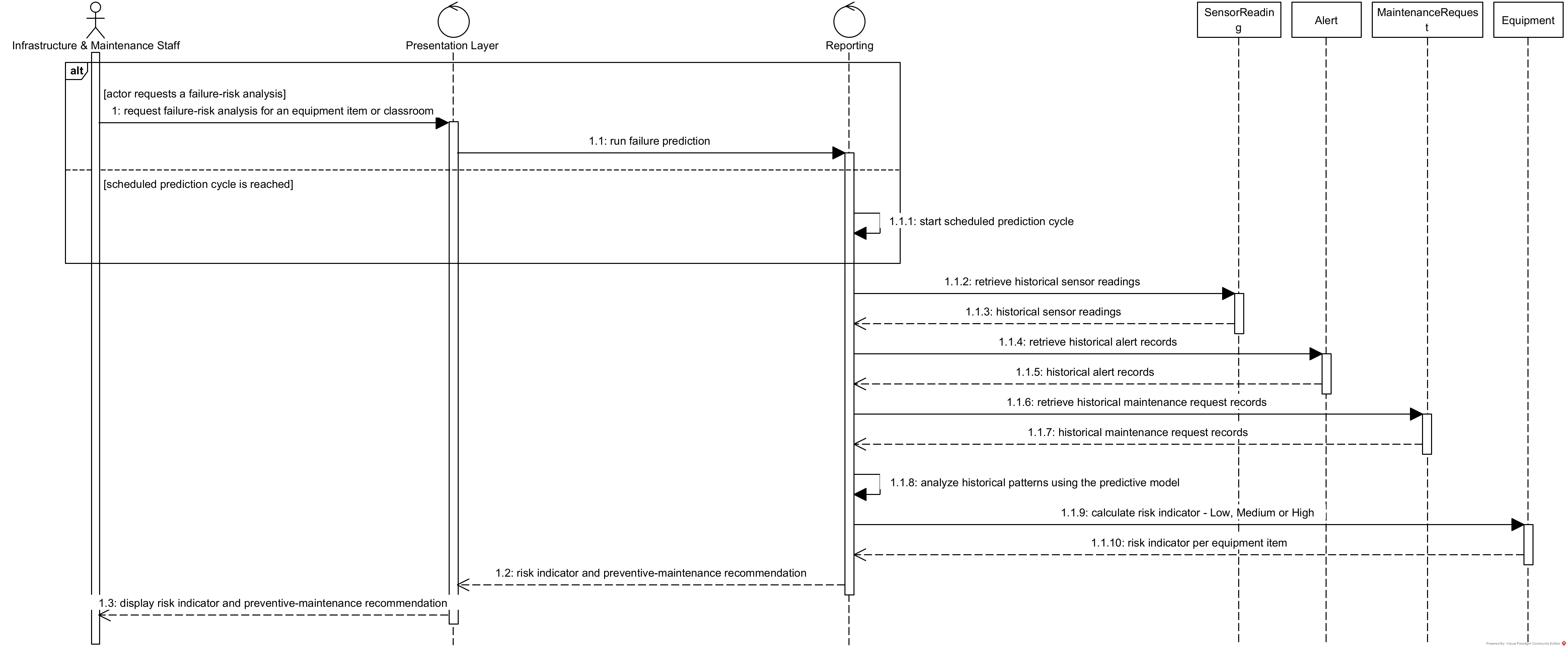
\includegraphics[width=1.25\textwidth]{seq_UC16_predict_equipment_failures.png}}
\caption{Diagrama de secuencia de CU-16, predicci\'on de fallas de equipos}
\label{fig:seq-uc16}
\end{figure}

\subsection{IA-02: An\'alisis de patrones de consumo energ\'etico (RF-14)}
\textbf{Tarea y tipo:} detecci\'on de anomal\'ias + agrupamiento no supervisado sobre series de consumo. \textbf{Sustenta:} RF-14, RF-17 (consumidor del resultado).

\textbf{(a) Descripci\'on del componente.} Entradas: ocupaci\'on (RF-03), estado de climatizaci\'on/proyector (RF-04/RF-05), lectura directa de consumo cuando exista sensor dedicado. Salida: lista de anomal\'ias de consumo (aula, franja horaria, magnitud), integrada al reporte administrativo (RF-17/RF-18). Consumidor: Autoridades de la Facultad, Personal Administrativo. \emph{Fallback:} una anomal\'ia mal detectada solo agrega una l\'inea a un reporte revisado por un humano; no ejecuta ninguna acci\'on sobre equipos.

\textbf{Requisitos funcionales del componente.} Los tres refinan RF-14 y alimentan RF-17; ninguno queda aislado.

\begingroup
\small
\begin{longtable}{|p{2.1cm}|p{9.4cm}|p{3.4cm}|}
\hline
\cellcolor{sigagreen}\textcolor{white}{\textbf{ID}} & \cellcolor{sigagreen}\textcolor{white}{\textbf{Enunciado verificable}} & \cellcolor{sigagreen}\textcolor{white}{\textbf{Traza}} \\ \hline
RF-IA-04 & El sistema debe calcular, para cada aula con al menos 60 d\'ias de historial, una l\'inea base de consumo por franja horaria y d\'ia de la semana, e indicar expl\'icitamente si esa l\'inea base proviene de un sensor de consumo real o del indicador indirecto (ocupaci\'on y estado de equipos). & Refina RF-14; se apoya en RF-03/RF-04/RF-05; verifica CP-IA-04 \\ \hline
RF-IA-05 & El sistema debe ejecutar, una vez al d\'ia, la detecci\'on de desviaciones respecto a la l\'inea base y producir la lista de anomal\'ias con aula, franja horaria y magnitud de la desviaci\'on. & Refina RF-14; verifica CP-IA-05; medido por RNF-IA-06, RNF-IA-07 y RNF-IA-08 \\ \hline
RF-IA-06 & El sistema debe incorporar las anomal\'ias detectadas al reporte administrativo del periodo, agregadas por aula y franja horaria, indicando para cada una la variable que m\'as contribuy\'o a la desviaci\'on. & Refina RF-14; alimenta RF-17/RF-18; operacionaliza RNF-IA-10 y RNF-IA-11; verifica CP-IA-06 \\ \hline
\caption{Requisitos funcionales del componente IA-02}
\end{longtable}
\endgroup

\textbf{(b) Datos de entrenamiento.} Volumen m\'inimo: 60 d\'ias por aula. No requiere etiquetado manual (modelo no supervisado). Sesgo conocido: las aulas sin sensor de consumo directo dependen de un indicador indirecto menos preciso: se declara expl\'icitamente en el reporte. Dato agregado de aula, no personal.

\textbf{(c) M\'etricas de \'exito.}
\begin{itemize}[nosep]
\item RNF-IA-06: tasa de falsos positivos $\leq$15\% sobre validaci\'on manual trimestral.
\item RNF-IA-07: an\'alisis por lote completado en $\leq$10 minutos, una vez al d\'ia.
\item RNF-IA-08: cobertura $\geq$90\% de las aulas con sensor de ocupaci\'on activo.
\end{itemize}

\textbf{(d) Requisitos \'eticos y de privacidad.}
\begin{itemize}[nosep]
\item RNF-IA-09 (equidad): diferencia de detecci\'on $\leq$15 puntos porcentuales entre aulas con y sin sensor de consumo real.
\item RNF-IA-10 (equidad): los reportes no atribuyen responsabilidad individual a un docente por consumo que no controla directamente (climatizaci\'on autom\'atica de RF-13); se reportan agregados por aula y franja.
\item RNF-IA-11 (explicabilidad): cada anomal\'ia indica la variable que m\'as contribuy\'o, sin requerir consulta t\'ecnica adicional.
\item Finalidad: eficiencia energ\'etica institucional, no evaluaci\'on individual. Sin identidad de usuario/docente. Ninguna acci\'on correctiva autom\'atica.
\end{itemize}

\textbf{(e) Plan de monitoreo.} Indicadores: falsos positivos mensuales, cobertura de aulas analizadas. Umbral de deriva: falsos positivos $>$25\% durante dos meses consecutivos, o cobertura $<$80\%. Reentrenamiento: recalcular l\'inea base al inicio de cada periodo acad\'emico.


\subsection{RNF-17: Seguridad f\'isica (Safety)}
\textbf{Nota de numeraci\'on:} el ERS ya usa el identificador RNF-16 (Disponibilidad en modo degradado sin conectividad, Fiabilidad, sustentado en EV-15). Este requisito nuevo se numera \textbf{RNF-17} para no colisionar.

\textbf{Descripci\'on cuantificada:} antes de ejecutar un apagado autom\'atico de climatizaci\'on (RF-13, RF-16), el sistema debe verificar que el aula est\'a efectivamente desocupada mediante al menos dos lecturas de sensor de presencia consecutivas, separadas por $\geq$30~s, y debe registrar en bit\'acora (RF-23) el estado de ocupaci\'on que motiv\'o cada apagado. Ante una lectura inconsistente o ausente, el sistema \textbf{no} debe ejecutar el apagado y debe generar una alerta de ``verificaci\'on fallida'' (fallback seguro).

\textbf{Caracter\'istica ISO/IEC 25010:2023:} Seguridad f\'isica (Safety).

\textbf{Criterio de verificaci\'on:} prueba de inyecci\'on de lecturas inconsistentes/ausentes durante un ciclo de apagado autom\'atico $\rightarrow$ el sistema no ejecuta el comando y genera la alerta en el 100\% de un m\'inimo de 20 casos de prueba.

\textbf{Estado de validaci\'on:} derivaci\'on directa de RD-04 y RF-13/RF-16: \textbf{borrador PE5, pendiente de validaci\'on de campo}; no existe evidencia de entrevista porque el guion aplicado en la Entrega 3 (2A) no incluy\'o preguntas sobre fallas de sensor durante apagados autom\'aticos.

\textbf{Trazas:} RF-13, RF-16, RD-04, RD-13.


\subsection{Comparaci\'on de los dos componentes}

Los dos componentes comparten el marco de especificaci\'on pero difieren en casi todo lo dem\'as, y esas diferencias tienen consecuencias de dise\~no que conviene hacer expl\'icitas (Tabla~\ref{tab:comparacion-ia}).

\begin{table}[H]
\centering
\small
\begin{tabular}{|p{3.1cm}|p{5.1cm}|p{5.1cm}|}
\hline
\cellcolor{sigagreen}\textcolor{white}{\textbf{Dimensi\'on}} & \cellcolor{sigagreen}\textcolor{white}{\textbf{IA-01 Predictor de fallas}} & \cellcolor{sigagreen}\textcolor{white}{\textbf{IA-02 Consumo energ\'etico}} \\ \hline
Tipo de aprendizaje & Supervisado, clasificaci\'on binaria & No supervisado, detecci\'on de anomal\'ias \\ \hline
Etiquetado & Autom\'atico, desde tickets correctivos cerrados & No requiere etiquetado \\ \hline
Historial m\'inimo & 90 d\'ias por equipo & 60 d\'ias por aula \\ \hline
Frecuencia & Diaria, con latencia $\leq$2 s por inferencia & Diaria, por lote, en $\leq$10 minutos \\ \hline
M\'etrica principal & F1 $\geq$0,70 en holdout temporal & Falsos positivos $\leq$15\,\% \\ \hline
Consumidor & Infraestructura y Mantenimiento & Autoridades y Personal Administrativo \\ \hline
Consecuencia de un error & Una alerta informativa de m\'as o de menos & Una l\'inea de m\'as o de menos en un reporte \\ \hline
Riesgo de equidad & Ignorar equipos de aulas poco usadas & Penalizar aulas con menos instrumentaci\'on \\ \hline
\end{tabular}
\caption{Comparaci\'on de los dos componentes de inteligencia artificial}
\label{tab:comparacion-ia}
\end{table}

La diferencia con mayor efecto sobre la especificaci\'on es la del etiquetado. IA-01 puede entrenarse sin trabajo manual porque el propio sistema genera su variable objetivo: un ticket correctivo cerrado con causa de falla \emph{es} la etiqueta. Esa comodidad tiene un costo que se declara en la ficha como sesgo conocido: el historial de fallas depende de cu\'an diligente fue el registro manual antes de que el sistema existiera, de modo que el modelo aprender\'a tambi\'en los h\'abitos de registro del personal, no solo el comportamiento de los equipos.

IA-02, en cambio, no necesita etiquetas pero arrastra un problema distinto: en las aulas sin sensor de consumo dedicado trabaja sobre un indicador indirecto (ocupaci\'on m\'as estado de equipos) que es menos preciso. De ah\'i que RF-IA-04 obligue a \textbf{declarar en el propio resultado} si la l\'inea base proviene de medici\'on real o de indicador indirecto: sin ese dato, un reporte mezclar\'ia dos calidades de evidencia sin que el lector pueda distinguirlas.

\subsection{Plan de monitoreo y criterio de retirada}

Ninguno de los dos componentes se declara terminado al desplegarse. Ambos tienen indicadores en producci\'on, frecuencia de medici\'on, umbral de deriva y criterio de reentrenamiento, que la Tabla~\ref{tab:monitoreo-ia} resume.

\begin{table}[H]
\centering
\small
\begin{tabular}{|p{2.9cm}|p{5.2cm}|p{5.2cm}|}
\hline
\cellcolor{sigagreen}\textcolor{white}{\textbf{Elemento}} & \cellcolor{sigagreen}\textcolor{white}{\textbf{IA-01}} & \cellcolor{sigagreen}\textcolor{white}{\textbf{IA-02}} \\ \hline
Indicadores & F1 mensual, falsos negativos por segmento, latencia p95 & Falsos positivos mensuales, cobertura de aulas analizadas \\ \hline
Umbral de deriva & Ca\'ida de F1 mayor a 15 puntos respecto a la l\'inea base & Falsos positivos por encima del 25\,\% durante dos meses, o cobertura bajo el 80\,\% \\ \hline
Reentrenamiento & Cada 90 d\'ias o al activarse el umbral & Al inicio de cada periodo acad\'emico \\ \hline
Retirada & Autom\'atica si F1 baja de 0,60 en dos evaluaciones consecutivas & No aplica: el resultado solo alimenta un reporte revisado por humanos \\ \hline
\end{tabular}
\caption{Plan de monitoreo de los componentes de inteligencia artificial}
\label{tab:monitoreo-ia}
\end{table}

La asimetr\'ia de la \'ultima fila es deliberada. IA-01 se retira solo porque una predicci\'on degradada genera alertas que consumen tiempo de personal t\'ecnico; dejarlo operando con F1 bajo tiene un costo real. IA-02 no necesita retirada autom\'atica porque su salida nunca llega a un actuador ni a una persona sin pasar antes por la revisi\'on de quien firma el reporte.

\subsection{Nota sobre el uso de modelos de lenguaje en el propio proceso}

Conviene distinguir dos usos de la inteligencia artificial en este proyecto, porque se eval\'uan de forma distinta. Uno es el de los componentes IA-01 e IA-02, que forman parte del sistema especificado y son objeto de esta secci\'on. El otro es el uso de modelos de lenguaje como asistente del propio proceso de ingenier\'ia de requisitos, que es lo que estudia el componente emp\'irico del proyecto y lo que se declara en el Anexo E. Sobre ese segundo uso existe hoy evidencia sistematizada acerca de su alcance y sus l\'imites \cite{cheng2026genai,arora2024advancing}, gu\'ias metodol\'ogicas para aplicarlo a tareas de procesamiento de lenguaje natural en requisitos \cite{vogelsang2024using}, y estudios espec\'ificos sobre elicitaci\'on asistida \cite{ronanki2023investigating,gorer2023generating}, aseguramiento de la calidad de requisitos \cite{lubos2024leveraging} y estandarizaci\'on de su redacci\'on \cite{ray2023agile}. Ninguno de esos trabajos sostiene que el modelo sustituya el an\'alisis humano, y este informe no lo asume.

\subsection{S\'intesis}

Ambos componentes se clasifican como riesgo m\'inimo/limitado bajo el enfoque del Reglamento (UE) 2024/1689, usado como marco de referencia de buenas pr\'acticas: no como obligaci\'on legal directa, dado que el sistema opera \'unicamente en Ecuador sin nexo con la Uni\'on Europea. La obligaci\'on legal real y aplicable es la Ley Org\'anica de Protecci\'on de Datos Personales del Ecuador \cite{asamblea2021lopdp}, cuyos art\'iculos 13 y 14 originan RF-24 y RF-25 y se mapean requisito por requisito en la \S3.4 del ERS. Ninguno de los dos componentes ejecuta una acci\'on autom\'atica irreversible sobre personas o equipos sin supervisi\'on humana: toda predicci\'on de alto riesgo o anomal\'ia de consumo pasa por revisi\'on de Infraestructura/Autoridades antes de generar un ticket o una decisi\'on de inversi\'on.

\section{M\'etricas de calidad}

\subsection{Tabla de auditor\'ia (plantilla 7.1 de la gu\'ia PE5)}

\begin{table}[H]
\centering
\small
\begin{tabular}{|p{4.2cm}|p{3.2cm}|p{2.9cm}|p{2.3cm}|c|}
\hline
\textbf{M\'etrica} & \textbf{Antes (v3.0)} & \textbf{Despu\'es (v4.0)} & \textbf{Referencia} & \textbf{Cumple} \\ \hline
M1a Completitud (4 atributos) & 70,73\,\% (29/41) & \textbf{100\,\% (42/42)} & $\geq$95\,\% & S\'i \\ \hline
M1b Completitud (CU) & 100\,\% (16/16) & 100\,\% (17/17) & 100\,\% & S\'i \\ \hline
M1c Actores con $\geq$1 RF & 100\,\% (9/9) & 100\,\% (9/9) & 100\,\% & S\'i \\ \hline
M2 Consistencia & 0,957 (2 abiertos) & \textbf{1,000 (0 abiertos)} & $\geq$0,98 y 0 abiertos & S\'i \\ \hline
M3 Verificabilidad & 100\,\% (41/41) & 100\,\% (42/42) & $\geq$90\,\% & S\'i \\ \hline
M4\_ade Trazabilidad adelante & 0\,\% (0/25) & \textbf{100\,\% (25/25)} & $\geq$90\,\% & S\'i \\ \hline
M4\_atr Trazabilidad atr\'as & 100\,\% (25/25) & 100\,\% (25/25) & 100\,\% & S\'i \\ \hline
M5 Modificabilidad & 4,2 & 4,2 & $\leq$3,0 & \textbf{No} \\ \hline
M6 Correcci\'on & 1,76 (72/41) & \textbf{0,00 (0/42)} & $\leq$0,05 & S\'i \\ \hline
\end{tabular}
\caption{Auditor\'ia de calidad del ERS: comparaci\'on antes/despu\'es}
\label{tab:auditoria-08}
\end{table}

Ocho de las nueve mediciones alcanzan su valor de referencia tras las correcciones (Tabla~\ref{tab:auditoria-08}). M5 no lo alcanza y no se maquilla: mide un acoplamiento real del dise\~no, no un defecto documental. Dos advertencias antes de leer las cifras, ambas desarrolladas m\'as abajo: M1c cambi\'o respecto del primer reporte porque se corrigi\'o la \emph{definici\'on operativa} que se estaba aplicando, no porque cambiara el documento; y M6 $=0{,}00$ significa ``cero defectos residuales \emph{de los registrados}'', con una re-inspecci\'on independiente todav\'ia pendiente.

\subsection{Operacionalizaci\'on de cada m\'etrica}

Antes de la aritm\'etica conviene fijar qu\'e cuenta como qu\'e, porque en varias m\'etricas el resultado depende m\'as de la definici\'on que del documento. La Tabla~\ref{tab:operacionalizacion} declara, para cada una, la unidad contada y el criterio de inclusi\'on aplicado.

\begin{table}[H]
\centering
\small
\begin{tabular}{|l|p{4.3cm}|p{6.6cm}|}
\hline
\cellcolor{sigagreen}\textcolor{white}{\textbf{M\'etrica}} & \cellcolor{sigagreen}\textcolor{white}{\textbf{Unidad contada}} & \cellcolor{sigagreen}\textcolor{white}{\textbf{Criterio de inclusi\'on aplicado}} \\ \hline
M1a & Requisito (25 RF + 17 RNF) & Se cuenta completo si tiene los cuatro atributos con contenido: identificador, prioridad, fuente y criterio de aceptaci\'on \\ \hline
M1b & Caso de uso (17) & Se cuenta especificado si tiene ficha textual con actores, prop\'osito, precondiciones, curso normal y flujos alternativos \\ \hline
M1c & Actor formal (9) & Se cuenta cubierto si participa en al menos un caso de uso, y por tanto en al menos un requisito que ese caso realiza \\ \hline
M2 & Verificaci\'on de coherencia (46) & Cada dato duplicado en dos o m\'as lugares cuenta como una verificaci\'on; un conflicto es una discrepancia entre esas apariciones \\ \hline
M3 & Criterio de verificaci\'on (42) & Se cuenta verificable si tiene umbral o resultado observable, unidad y m\'etodo, y no contiene vocabulario no medible \\ \hline
M4\_ade & Requisito funcional (25) & Cadena completa si se recorre RF $\rightarrow$ CU $\rightarrow$ clase $\rightarrow$ estado $\rightarrow$ prueba, contando el estado como satisfecho si la entidad no tiene ciclo de vida \\ \hline
M4\_atr & Requisito funcional (25) & Se cuenta trazado si el campo de origen identifica una evidencia, norma o an\'alisis \\ \hline
M5 & Requisito de la muestra (5) & Un requisito est\'a acoplado a otro si comparten al menos un caso de uso o una clase de dominio \\ \hline
M6 & Instancia de defecto (71) & Cuentan las contradicciones, atributos faltantes y ambig\"uedades sobre requisitos ya escritos; no cuentan los artefactos que la Unidad V manda construir \\ \hline
\end{tabular}
\caption{Unidad contada y criterio de inclusi\'on de cada m\'etrica}
\label{tab:operacionalizacion}
\end{table}

La fila de M1c y la de M4\_ade son las dos que admiten una lectura alternativa defendible, y por eso ambas se discuten expl\'icitamente m\'as abajo con el valor que arrojar\'ia esa lectura.

\subsection{Aritm\'etica y m\'etodo}

\textbf{M1a.} Antes: 25/25 fichas RF completas, pero solo 4/16 RNF, porque solo NFR-01, 02, 03 y 10 ten\'ian prioridad MoSCoW. Correcci\'on: se declar\'o la prioridad de los 13 RNF pendientes en la Tabla 42, cada una con justificaci\'on escrita (7 Must, 5 Should, 1 Could). El criterio aplicado fue: Must lo que, de faltar, impide operar o expone a incumplimiento legal; Should lo que degrada la calidad sin bloquear; Could lo que solo facilita la evoluci\'on futura. Despu\'es: $42/42$, es decir 100\,\%.

\textbf{M1c: correcci\'on de la definici\'on operativa.} El primer reporte aplic\'o la lectura ``actores que \emph{originan} al menos un RF'' y midi\'o $2/9$, es decir 22,22\,\%. Esa lectura es incorrecta por una raz\'on concreta: convierte M1c en un duplicado de M4\_atr, que ya mide exactamente eso. La lectura literal de la f\'ormula, ``\#actores con $\geq$1 RF'', es de \textbf{cobertura}: ning\'un actor debe quedar sin funcionalidad asociada. Verificado por conteo sobre los 17 CU, los nueve actores participan en al menos uno: desde Personal de Infraestructura (10 CU) hasta Sistema de Videovigilancia (1 CU), luego $9/9$, es decir 100\,\%. La concentraci\'on de fuentes de elicitaci\'on que revelaba la otra lectura no desaparece: se mantiene declarada como limitaci\'on de validez (D-03).

\textbf{M2.} Definici\'on operativa: coherencia de cada requisito contra todas sus declaraciones duplicadas: prioridad de los 42 requisitos contrastada entre Tabla 42, \S5.2 y el CSV (42 comparaciones), conteos narrativos frente a identificadores definidos (3) y alcance del MVP entre \S6.1 y \S6.4 (1). Total 46 verificaciones, 2 conflictos hallados (D-01 y D-12), ambos cerrados: $1-0/46 = 1{,}000$. \emph{Limitaci\'on declarada:} no se ejecut\'o el barrido sem\'antico par a par de los 400 pares RF$\leftrightarrow$RNF; un conflicto de contenido latente no quedar\'ia capturado por esta medici\'on.

\textbf{M3.} Cero t\'erminos no medibles en los 42 criterios de verificaci\'on, incluido el nuevo RNF-17, cuyo criterio fija 20 casos de prueba y un 100\,\% de aciertos exigido.

\textbf{M4\_ade.} Cadena \texttt{RF} $\rightarrow$ \texttt{CU} $\rightarrow$ \texttt{clase} $\rightarrow$ \texttt{estado} $\rightarrow$ \texttt{prueba}, contando ``estado'' como satisfecho cuando la entidad no tiene ciclo de vida modelado (la plantilla 7.2 lo marca ``si aplica''). Antes $0/25$, por inexistencia de casos de prueba y de DFD; despu\'es $25/25$. La cadena extendida que adem\'as exige criterio BDD cierra en $17/25$, es decir 68\,\%, porque solo los RF Must llevan historia y Gherkin, que es lo que la gu\'ia pide.

\textbf{M5.} Recalculado por script sobre la matriz: acoplamiento de 6, 6, 5, 2 y 2 para RF-01, RF-07, RF-13, RF-19 y RF-24. Promedio $21/5 = 4{,}2$, sin cambio. Se comprob\'o si la creaci\'on de CU-17 desacoplaba a RF-24 y \textbf{no lo hace}: sigue unido a RF-19 por la clase \texttt{Usuario}. Bajar de 3,0 exigir\'ia rediseñar el modelo de dominio, no reescribir requisitos, y eso excede el alcance de una unidad de ingenier\'ia de requisitos.

\textbf{M6.} Se cuentan solo defectos de calidad de requisitos preexistentes; la columna \texttt{Cuenta\_para\_M6} del registro marca cu\'ales entran, excluyendo los artefactos que la propia gu\'ia manda construir en la PE5. Antes: D-01 (3) + D-02 (12) + D-06 (3) + D-09 (16) + D-10 (17) + D-12 (1) + D-13 (17) + D-14 (2) $= 71/41 = 1{,}73$. Despu\'es: $0/42 = 0{,}00$. El denominador cambia de 41 a 42 porque la versi\'on 4.0 incorpora RNF-17.

\subsection{Advertencia sobre el M6 igual a cero}

Un 0,00 no significa que el ERS carezca de defectos: significa que no queda ninguno \textbf{de los registrados}. La re-inspecci\'on posterior fue automatizada y verific\'o lo comprobable por script: conteos, identificadores definidos, coherencia de prioridad entre tablas y CSV, cobertura de historias de los 17 Must, balance de entornos LaTeX, pero una re-lectura sem\'antica completa \textbf{por una persona distinta de quien aplic\'o las correcciones} sigue pendiente, y es lo que dar\'ia a este valor su respaldo definitivo. Declararlo de otro modo ser\'ia el error que la propia gu\'ia advierte: reportar correcci\'on total cuando el anexo no la respalda.

\subsection{Amenazas a la validez de esta medici\'on}

Las cifras de la Tabla~\ref{tab:auditoria-08} son reproducibles, pero eso no las hace inmunes a sesgo. Se declaran cuatro amenazas concretas:

\textbf{El auditor y el corrector son la misma parte.} Quien detect\'o los defectos aplic\'o tambi\'en las correcciones y volvi\'o a medir. Es la amenaza m\'as seria del conjunto y afecta sobre todo a M6: no hay ninguna garant\'ia de que una lectura externa no encuentre defectos que esta pas\'o por alto. La evidencia de \S5 (dos defectos aparecidos en la segunda pasada) sugiere que probablemente los haya.

\textbf{Varias m\'etricas dependen de una definici\'on operativa elegida por el equipo.} M1c cambia de 22\,\% a 100\,\% seg\'un se lea ``actores que originan un RF'' o ``actores cubiertos por al menos un RF''; M4\_ade depende de que ``estado'' se cuente como satisfecho cuando la entidad no tiene ciclo de vida. Ambas elecciones est\'an argumentadas y declaradas, pero un evaluador que adopte la lectura contraria obtendr\'a otros n\'umeros. Por eso se reporta en cada caso el valor alternativo.

\textbf{M5 se calcula sobre una muestra, no sobre el conjunto.} Cinco requisitos de veinticinco, elegidos por representatividad funcional y no al azar. La gu\'ia admite expresamente una muestra de al menos cinco, pero la elecci\'on intencional puede favorecer o perjudicar el promedio; con RF de \'areas menos acopladas el valor bajar\'ia.

\textbf{La consistencia se verific\'o sobre declaraciones, no sobre sem\'antica.} Las 46 comprobaciones de M2 detectan que dos lugares del documento digan cosas distintas del mismo elemento. No detectan que dos requisitos, cada uno internamente coherente, sean incompatibles entre s\'i en su contenido. Un conflicto de ese tipo seguir\'ia latente.

\subsection{Qu\'e queda pendiente}

M5 (4,2 frente a $\leq$3,0), que se asume y se justifica; la re-inspecci\'on independiente de la versi\'on 4.0; el barrido sem\'antico par a par que cerrar\'ia la limitaci\'on de M2; y ampliar la elicitaci\'on a los siete actores nunca entrevistados como fuente (D-03).

\section{Retrospectiva}

La Tabla~\ref{tab:retro} recoge la retrospectiva en formato Start--Stop--Continue (Anexo D de la gu\'ia PE5), con responsable por cada acci\'on de mejora.

\begin{table}[H]
\centering
\small
\begin{tabular}{|l|p{9cm}|l|}
\hline
\textbf{Categor\'ia} & \textbf{Elemento} & \textbf{Responsable} \\ \hline
\multirow{3}{*}{Start} & Ejecutar una auditor\'ia de calidad real (con conteo verificable) al cierre de cada entrega, no solo al final del curso: esta PE5 fue la primera inspecci\'on formal jam\'as registrada del proyecto. & Verificador \\ \cline{2-3}
 & Sincronizar el archivo de priorizaci\'on MoSCoW con el cuerpo del ERS en cada cambio, y registrar el porqu\'e de cada reclasificaci\'on: evita contradicciones como D-01. & Analista l\'ider \\ \cline{2-3}
 & Etiquetar (\texttt{git tag}) la l\'inea base del ERS al cierre de cada entrega, para tener puntos de comparaci\'on reales entre versiones. & Equipo \\ \hline
\multirow{3}{*}{Stop} & Editar el archivo de priorizaci\'on (CSV) sin sincronizar el cambio con el cuerpo del ERS: caus\'o la contradicci\'on D-01 (RF-20/24/25) que bloque\'o varias m\'etricas. & Equipo \\ \cline{2-3}
 & Dejar los RNF fuera de la matriz de trazabilidad mientras se traza minuciosamente cada RF: caus\'o que 16 RNF quedaran sin fila propia (D-09). & Documentadora \\ \cline{2-3}
 & Redactar historias de usuario con una cl\'ausula ``Cuando'' gen\'erica de plantilla en vez del evento real que dispara el escenario (D-10). & Modeladores \\ \hline
\multirow{3}{*}{Continue} & Declarar expl\'icitamente lo que no est\'a validado (``No verificado (ver Secci\'on X'') en vez de maquillar un porcentaje) pr\'actica ya presente en el ERS desde la Entrega 3 (2A) y que esta unidad mantiene. & Equipo \\ \cline{2-3}
 & Mantener la plantilla de 8 atributos para cada RF: dio 100\% de completitud real en esta auditor\'ia (M1a sobre RF). & Modeladores \\ \cline{2-3}
 & Citar la evidencia de campo exacta (EV-xx) en cada requisito: es lo que permiti\'o M4\_atr = 100\% en esta auditor\'ia. & Documentadora \\ \hline
\end{tabular}
\caption{Retrospectiva Start-Stop-Continue}
\label{tab:retro}
\end{table}

\subsection{Lectura de la retrospectiva}

Las nueve entradas de la Tabla~\ref{tab:retro} no son impresiones: cada una se apoya en un defecto registrado o en una m\'etrica de \S8. Conviene explicar las tres que m\'as cambiar\'ian el resultado si se hubieran aplicado antes.

\textbf{Auditar al cierre de cada entrega, no solo al final (Start).} Es la de mayor retorno. El proyecto acumul\'o setenta y una instancias de defecto a lo largo de tres versiones porque nunca hubo un instrumento de medici\'on hasta la Unidad V. Ninguno de esos defectos era dif\'icil de encontrar: D-01 se detecta comparando dos archivos, D-02 contando campos vac\'ios. El costo de haberlos arrastrado no fue el de corregirlos (eso llev\'o horas) sino el de haber construido modelos, historias y un MVP sobre una priorizaci\'on que se contradec\'ia a s\'i misma.

\textbf{Dejar de editar un artefacto sin sincronizar sus duplicados (Stop).} Los tres defectos de contradicci\'on del registro: D-01, D-12 y D-14: comparten causa: un dato que vive en dos lugares y se actualiz\'o en uno solo. La prioridad MoSCoW viv\'ia en la Tabla 42 y en un CSV; el alcance del MVP, en las secciones 6.1 y 6.4; la caracter\'istica de calidad, en la Tabla 39 y en la declaraci\'on de cobertura de la norma. La acci\'on correctiva no es ``tener m\'as cuidado'', que no es accionable, sino reducir la duplicaci\'on: la priorizaci\'on qued\'o consolidada en un \'unico archivo y esa es la raz\'on por la que se elimin\'o el duplicado en lugar de mantener los dos sincronizados.

\textbf{Mantener la declaraci\'on expl\'icita de lo no validado (Continue).} Es la pr\'actica que m\'as sostiene la credibilidad del ERS ante el tribunal, y viene de la Entrega 3. Nueve de los diecisiete RNF siguen marcados como ``no verificado'' con la raz\'on escrita al lado. La tentaci\'on de reetiquetarlos como validados al cerrar el proyecto existi\'o y se descart\'o: un umbral que nadie midi\'o no se vuelve cierto porque el documento lo afirme, y un anexo que lo desmienta cuesta m\'as que el pendiente declarado.

\subsection{Lo que esta retrospectiva no puede cerrar}

Dos de las acciones de mejora exceden el alcance de una unidad y se dejan enunciadas sin responsable de cierre. La primera es la ampliaci\'on de las fuentes de elicitaci\'on: depende de la disponibilidad de personas, no de esfuerzo del equipo. La segunda es la reducci\'on del acoplamiento que mide M5, que exigir\'ia rediseñar el modelo de dominio (separar el agregado \texttt{Aula} de \texttt{LecturaSensor}) y por tanto rehacer buena parte del modelado UML y de la matriz. Ambas quedan como recomendaci\'on para una eventual continuaci\'on del proyecto, no como compromiso de esta entrega.

\section{Conclusiones}

Se presenta una conclusi\'on por unidad. Cada una enuncia un hallazgo que este proyecto produjo y que no ser\'ia igual de v\'alido en otro: una afirmaci\'on que podr\'ia aparecer en cualquier informe no es una conclusi\'on.

\subsection{Unidad I: Planificaci\'on y elicitaci\'on}

Aplicar tres t\'ecnicas de elicitaci\'on distintas produjo resultados consistentes en el n\'ucleo funcional: entrevista, cuestionario y observaci\'on directa convergieron en los mismos RF-01 a RF-13. Esa convergencia se interpret\'o en su momento como se\~nal de cobertura suficiente, y la auditor\'ia de la Unidad V mostr\'o que era una lectura incompleta. Las tres t\'ecnicas se aplicaron mayoritariamente sobre las mismas dos fuentes, de modo que su acuerdo mide consistencia de esas fuentes, no cobertura del dominio: siete de los nueve actores del sistema nunca fueron origen de un requisito. \textbf{La diversidad de t\'ecnicas no sustituye a la diversidad de informantes}, y confundirlas produce una falsa sensaci\'on de saturaci\'on. En este proyecto la limitaci\'on es de poblaci\'on: el conjunto de personas que operan las aulas es reducido y el docente autoriz\'o cerrar en once entrevistas, pero la lecci\'on metodol\'ogica se sostiene con independencia de esa autorizaci\'on.

\subsection{Unidad II: Especificaci\'on}

La decisi\'on de exigir umbral, unidad y m\'etodo de comprobaci\'on en cada criterio de aceptaci\'on desde la primera redacci\'on tuvo un retorno medible: la verificabilidad result\'o 100\,\% en la auditor\'ia, sin una sola reescritura correctiva. Es la \'unica de las nueve mediciones que naci\'o cumpliendo su umbral. El contraste con lo ocurrido en las historias de usuario es instructivo: all\'i donde se us\'o una plantilla que se rellenaba mec\'anicamente: la cl\'ausula ``cuando se cumple la condici\'on operativa de RF-XX'': el resultado fueron diecisiete escenarios inservibles como criterio de prueba. \textbf{Una plantilla disciplina la redacci\'on solo si cada campo obliga a una decisi\'on}; si admite un relleno gen\'erico, produce documentos que parecen completos y no lo est\'an.

\subsection{Unidad III: Modelado}

El modelado UML fue exhaustivo en las dos dimensiones que la asignatura enfatiza: estructura (clases, componentes, despliegue) y comportamiento: secuencia, actividad, estados, con m\'as de cuarenta diagramas. Ninguno describ\'ia el flujo de datos a nivel de proceso. Ese hueco no se detect\'o durante tres entregas consecutivas porque cada modelo era correcto por separado y la revisi\'on se hizo modelo por modelo. Solo apareci\'o al intentar recorrer la cadena de trazabilidad completa, que exige un eslab\'on de proceso entre la clase y la prueba. \textbf{La completitud de un conjunto de modelos no se verifica revis\'andolos uno a uno, sino intentando atravesarlos de extremo a extremo}: la traza es el instrumento que detecta la vista ausente.

\subsection{Unidad IV: Validaci\'on}

Este proyecto lleg\'o a la Unidad V con tres versiones del ERS, una calificaci\'on de 9,70/10 en la Entrega 2 y \emph{cero} registros de inspecci\'on. La primera inspecci\'on formal, hecha en esta unidad, encontr\'o catorce defectos ra\'iz y setenta y una instancias, entre ellas una contradicci\'on cr\'itica de prioridad que hab\'ia sobrevivido a las tres versiones. Ninguno de esos defectos era sutil; simplemente nadie los hab\'ia buscado con un instrumento. \textbf{Un documento revisado no es un documento inspeccionado}: la revisi\'on informal confirma lo que el autor cree haber escrito, mientras que la inspecci\'on con criterios fijados de antemano contrasta el documento con una definici\'on externa de correcci\'on.

\subsection{Unidad V: Integraci\'on, m\'etricas y defensa}

Medir sobre el documento real, y no sobre una estimaci\'on de c\'omo deber\'ia verse, corrigi\'o el diagn\'ostico del proyecto en las dos direcciones: elev\'o una m\'etrica que se supon\'ia d\'ebil (la verificabilidad result\'o 100\,\%) y confirm\'o con evidencia exacta una debilidad que solo se intu\'ia. M\'as revelador a\'un fue el efecto de las definiciones: M1c pas\'o de 22\,\% a 100\,\% sin que el documento cambiara una l\'inea, solo por corregir la lectura operativa de la f\'ormula. \textbf{Una m\'etrica sin definici\'on operativa expl\'icita no mide calidad, mide la interpretaci\'on de quien la calcula}, y por eso el valor de una auditor\'ia est\'a menos en el n\'umero que en la aritm\'etica reproducible que lo acompa\~na. Es tambi\'en la raz\'on por la que este informe declara sus cuatro amenazas a la validez (\S8) en lugar de presentar nueve cifras cerradas.

\subsection{Conclusi\'on integradora}

Las cinco unidades comparten un mismo patr\'on: en cada una, el artefacto que parec\'ia terminado result\'o incompleto en cuanto se lo someti\'o a un instrumento externo: otro informante, otra plantilla, otra traza, otra lista de verificaci\'on, otra definici\'on. El aprendizaje central del Proyecto Integrador no es que la ingenier\'ia de requisitos produzca documentos, sino que \textbf{la calidad de un requisito no es una propiedad del texto, sino del proceso de contraste al que ese texto ha sido sometido}. Un ERS con veinticinco requisitos bien redactados y ninguna inspecci\'on registrada tiene menos garant\'ias que uno con defectos conocidos, ubicados y contados.


% =====================================================================
% REFERENCIAS
% =====================================================================
\newpage
\printbibliography[title={IX. Referencias}]

% =====================================================================
% ANEXOS
% =====================================================================
\newpage
\section*{Anexos}
\addcontentsline{toc}{section}{Anexos}

\subsection*{Anexo A: Instrumento de auditor\'ia de calidad del ERS}
\addcontentsline{toc}{subsection}{Anexo A: Instrumento de auditor\'ia de calidad del ERS}

Ver \S5 y \S8 de este informe para la tabla de auditor\'ia y la aritm\'etica completa. El detalle l\'inea por l\'inea, con los comandos exactos usados para reproducir cada conteo, est\'a en los dos archivos que la carpeta \texttt{09\_Metricas/} del repositorio contiene: el anexo de auditor\'ia en formato Markdown y el registro de defectos en formato CSV.

\textbf{Instrumento aplicado.} Para cada m\'etrica se registra la f\'ormula, los conteos usados, el resultado, el valor de referencia, el veredicto y la acci\'on de mejora, conforme a la escala de valoraci\'on de la gu\'ia que recoge la Tabla~\ref{tab:escala-auditoria}:

\begin{table}[H]
\centering
\small
\begin{tabular}{|c|p{11.0cm}|}
\hline
\textbf{Nivel} & \textbf{Criterio} \\ \hline
4 & Cumple el valor de referencia con evidencia completa \\ \hline
3 & Lo cumple con evidencia parcial \\ \hline
2 & Queda por debajo, pero con acci\'on de mejora documentada y aplicada \\ \hline
1 & Queda por debajo sin acci\'on \\ \hline
0 & No se midi\'o \\ \hline
\end{tabular}
\caption{Escala de valoraci\'on por m\'etrica del instrumento de auditor\'ia}
\label{tab:escala-auditoria}
\end{table}

Aplicada a los resultados de \S8, la valoraci\'on es de nivel 4 en M1a, M1b, M1c, M2, M3, M4 y M6, y de nivel 2 en M5: queda por debajo del umbral, pero con la causa identificada (acoplamiento del modelo de dominio), la acci\'on de mejora enunciada (separar el agregado \texttt{Aula} de \texttt{LecturaSensor}) y la raz\'on por la que no se aplic\'o en esta unidad (exige rehacer el modelado UML y la matriz completos).

\subsection*{Anexo B: Banco de preguntas del tribunal}
\addcontentsline{toc}{subsection}{Anexo B: Banco de preguntas del tribunal}

Reproducido de la Gu\'ia Ampliada PE5 (\S10, Anexo B), con la respuesta anticipada de cada tema y el artefacto que la respalda.

\begin{table}[H]
\centering
\small
\begin{tabular}{|l|p{10cm}|}
\hline
Fundamentos & \S1--3: frontera del sistema y l\'imite; diferencia contexto/l\'imite en este proyecto; modelo de proceso seguido y por qu\'e. \\ \hline
Elicitaci\'on & \S4--6: t\'ecnica que aport\'o requisitos no descubribles de otro modo; stakeholder subrepresentado (respuesta lista: los 7 actores sin RF de origen, D-03) y c\'omo se compens\'o; origen concreto de un requisito. \\ \hline
Especificaci\'on & \S7--9: un RNF elegido y c\'omo se comprueba objetivamente; el requisito m\'as costoso de redactar verificable; por qu\'e un CU incluye a otro y no lo extiende. \\ \hline
Validaci\'on & \S10--12: cu\'antos defectos hall\'o la inspecci\'on y cu\'ales siguen abiertos (respuesta lista: 14 defectos ra\'iz, 71 instancias contables; los que cuentan para M6 quedaron cerrados y se mantiene declarada la limitaci\'on de elicitaci\'on D-03); qu\'e defecto cr\'itico se escap\'o y c\'omo se detect\'o (D-01, contradicci\'on de MoSCoW entre el ERS y el CSV de priorizaci\'on, que sobrevivi\'o tres versiones porque nunca hubo inspecci\'on); c\'omo se sabe que las correcciones no introdujeron nuevos defectos (se volvi\'o a medir: M4\_ade 0\,\%$\rightarrow$100\,\% y M6 1,73$\rightarrow$0,00, con la advertencia de \S8.4 sobre la re-inspecci\'on pendiente). \\ \hline
Gesti\'on & \S13--15: qu\'e RF se rompe si ma\~nana cambia (usar la muestra M5: RF-01/RF-07 afectan a 6 otros RF cada uno); qu\'e RFC rechaz\'o el CCB (respuesta honesta: no existi\'o un CCB formal documentado en ninguna entrega, se declara como vac\'io de proceso); l\'inea base vigente y d\'onde est\'a etiquetada (commit \texttt{9f7c54c}, sin tag de Git formal: pendiente). \\ \hline
IA & \S16--18: qu\'e decide el modelo y qu\'e pasa cuando se equivoca (ver fichas IA-01/IA-02, bloque (a), fallback); con qu\'e datos se entrenar\'ia y con qu\'e base legal (bloque (b) de cada ficha); c\'omo se medir\'ia que el modelo no perjudica sistem\'aticamente a un grupo (RNF-IA-04/05/09/10, equidad). \\ \hline
M\'etricas & \S19--20: qu\'e m\'etrica sali\'o peor y qu\'e se hizo (M4\_ade sali\'o 0\,\%; se construyeron el DFD, CU-17 y los 42 casos de prueba en esta unidad y volvi\'o a medirse en 100\,\%. La peor al cierre es M6, 0,73 frente a un umbral de 0,05); mostrar los conteos de verificabilidad (M3, 41/41, comando de b\'usqueda documentado en \S8.2). \\ \hline
\'Etica & \S21--22: qu\'e datos personales trata el sistema y c\'omo se protegen (credenciales, bit\'acora; AES-256, NFR-03; CU-17 para derechos ARCO); qu\'e partes de este informe fueron asistidas por IA y c\'omo se validaron (ver Anexo E). \\ \hline
\end{tabular}
\end{table}

\subsection*{Anexo C: Declaraci\'on individual de aporte al PFC}
\addcontentsline{toc}{subsection}{Anexo C: Declaraci\'on individual de aporte al PFC}

\textbf{Aporte hist\'orico verificable (PE1--PE4, hasta el 02/08/2026), seg\'un el historial real de \texttt{git log} de ambos repositorios: ninguna cifra de esta tabla est\'a estimada:}

\begin{table}[H]
\centering
\small
\begin{tabular}{|p{4.6cm}|c|c|p{5.4cm}|}
\hline
\textbf{Integrante} & \textbf{ERS} & \textbf{MVP} & \textbf{Aportes concretos verificables} \\ \hline
S\'anchez Cornejo Gary Alberto & 50 & 4 & Estructura del repositorio, MVP completo, evidencias e integraci\'on general \\ \hline
Mu\~noz Qui\~nonez Yeranick Esther & 24 & 0 & Evidencias de campo y transcripciones \\ \hline
Mendoza Palma Allan Jeremy & 19 & 0 & Diagramas UML de actividad y secuencia, evidencias \\ \hline
Cede\~no Avila Winston Damian & 16 & 0 & Diagramas UML de componentes y despliegue, evidencias \\ \hline
Gilces Carranza Jos\'e Ignacio & 0 & 0 & Ninguno verificable en el historial hasta el 20/08/2026 \\ \hline
\end{tabular}
\caption{Aporte hist\'orico PE1--PE4 (fuente: \texttt{git log --format="\%an"} de ambos repositorios)}
\end{table}

\textbf{Aporte en la Unidad V (PE5):} S\'anchez Cornejo Gary Alberto, Mu\~noz Qui\~nonez Yeranick Esther, Ce\~no Avila Winston Damian y Mendoza Palma Allan Jeremy son los integrantes activos del equipo en esta unidad. Gilces Carranza Jos\'e Ignacio no registra aporte verificable, ni en las entregas anteriores ni en la Unidad V. Esta tabla se completa con el detalle de aporte de la PE5 una vez existan los commits correspondientes sobre esta carpeta.

\subsection*{Anexo D: Retrospectiva}
\addcontentsline{toc}{subsection}{Anexo D: Retrospectiva}

Ver \S9 de este informe.

\subsection*{Anexo E: Referencias y declaraci\'on de uso de IA}
\addcontentsline{toc}{subsection}{Anexo E: Referencias y declaraci\'on de uso de IA}

\textbf{Herramienta:} Claude (Anthropic), modelo Opus 5, v\'ia Claude Code, sesiones del 20 al 22 de agosto de 2026.

\textbf{Secciones asistidas y tipo de asistencia:}
\begin{itemize}[nosep]
\item \textbf{Auditor\'ia de calidad (Anexo A, \S5, \S8):} extracci\'on de conteos reales del documento (grep/awk sobre el .tex y los .csv reales), c\'alculo de las f\'ormulas de la gu\'ia sobre esos conteos, y redacci\'on de la interpretaci\'on. Los conteos son reproducibles con los comandos documentados en el Anexo A; no se gener\'o ning\'un n\'umero sin poder mostrarlo.
\item \textbf{Fichas de IA (IA-01, IA-02) y RNF-17:} redacci\'on completa asistida por IA, a partir del dominio real del sistema (RF-09, RF-14, RF-13/RF-16 ya existentes en el ERS). No se cit\'o ninguna evidencia de campo (EV-xx) que no existiera; donde no hay evidencia real, se declara expl\'icitamente ``borrador PE5, pendiente de validaci\'on de campo''.
\item \textbf{DFD Nivel 1, CU-17, matriz de trazabilidad PE5, registro de hu\'erfanos:} construcci\'on completa asistida por IA, derivada del modelo real de RF/CU/clases ya existente en el ERS y en \texttt{matriz\_trazabilidad.csv}: no de una plantilla gen\'erica.
\item \textbf{Retrospectiva (\S9) y Conclusiones (\S10):} redacci\'on asistida por IA a partir de hechos verificables del repositorio (fechas, versiones, hallazgos de la auditor\'ia).
\end{itemize}

\textbf{M\'etodo de validaci\'on del contenido:} toda cifra de m\'etrica y todo defecto reportado en este informe es reproducible ejecutando los comandos documentados en el Anexo A sobre el repositorio real (\texttt{github.com/gsanchezc6-beep/SIGA\_FGMMN\_ISR401\_AVANCE\_2A}, commit \texttt{9f7c54c}). Ninguna secci\'on evaluativa (conclusiones, justificaciones de decisiones de ingenier\'ia) se declara como producci\'on \'integra de IA sin revisi\'on humana subsecuente.


\end{document}
